\documentclass[a4paper,10pt]{article}

\usepackage[margin=1in]{geometry} 	% Setea el margen manualmente, todos iguales.
\usepackage[spanish]{babel} 		% {Con estos dos anda
\usepackage[utf8]{inputenc} 		% todo lo que es tildes y ñ}
\usepackage{fancyhdr} 			%{Estos dos son para
\pagestyle{fancyplain} 			% el header copado}
\usepackage{color}			% Con esto puedo hacer la matufia de poner en color blanco un texto para engañar al formato
\usepackage{xcolor,graphicx}
\usepackage{hyperref}

\lhead{Sistemas Operativos}% {Con esto se usa el header copado. También está \chead para
\rhead{Trabajo Práctico Número 1} 	% el centro y comandos para el pie de página, buscar fancyhdr}


%%%%%%%%%%%%%%%%%%%%%%%%%%%%%%%%%%%%%
%      COMANDOS ÚTILES USADOS       %
%%%%%%%%%%%%%%%%%%%%%%%%%%%%%%%%%%%%%

% \section{title} 		Te hace un título ``importante'' en negrita, numerado. También está \subsection{title} y \subsubsection{title}.
% \begin{itemize}		Te hace viñetas.
%	\item esto es un item	Cambiar itemize por enumerate te hace una numeración.
% \end{itemize}

% \textbf{text} 		Te hace el texto en negrita (bold).
% \underline{text}		Te subraya el texto.

% \textsuperscript{text}	Te hace ``superindices'' con texto. En teoría subscript debería funcionar, pero se puede usar guion bajo entre llaves
% 				y signos peso para hacerlo como alternativa. Sino buscar.

% \begin{tabular}{cols} 	Es para hacer tablas. Se pone una c por cada columna deseada dentro de cols (si es que se desea centrada, l para justificar a 
%	a & b & c		izquierda, r a la derecha). Si se separa por espacios la tabla no tendrá líneas divisorias. Si se separa por | en lugar de 
% \end{tabular}			espacios, aparecerá una línea. Con || dos, y así. Luego para los elementos de las filas se escriben y se separan con ampersand (&).
%				Finalmente, para las líneas horizontales, se usa \hline para una linea en toda la tabla y \cline{i - j} te hace la linea desde
%				la celda i hasta la j, arrancando en 1.
%				Si en la columna se pone p(width) podés escribir un párrafo en la celda. Para hacer un enter con \\ no funciona porque te hace un
%				enter en la fila. Para eso se usa el comando \newline.
  
% \textcolor{color predefinido en palabras}{text}

%%%%%%%%%%%%%%%%%%%%%%%%%%%%%%%%%%%%%
%    FIN COMANDOS ÚTILES USADOS     %
%%%%%%%%%%%%%%%%%%%%%%%%%%%%%%%%%%%%%

\begin{document}

%%%%%%%%%%%%%%%%%%%%%%%%%%%%%%
%    Carátula										      %
%%%%%%%%%%%%%%%%%%%%%%%%%%%%%%

\begin{titlepage}
\begin{center}

\textnormal{Universidad de Buenos Aires}\\
\textnormal{Facultad de Ciencias Exactas y Naturales}\\
\textnormal{Departamento de Computación}\\

\vspace{5cm}

\large\textbf{Sistemas Operativos - Primer cuatrimestre 2013} \\
\textbf{Trabajo Práctico Número 1\\
Scheduling} \\

\vspace{5cm}

\begin{tabular}{|c c c|} \hline
  L.U. & Integrante & E-Mail \\ \hline
  125/10 & Giordano, Mauro & mauro.foxh@gmail.com \\ \newline
  039/10 & Tastzian, Juan Manuel & jm@tast.com.ar \\ \newline
  500/10 & Vallejo, Nicolás Agustín & nicopr08@gmail.com \\ \hline
\end{tabular}

\end{center}


\end{titlepage}
\newpage

%%%%%%%%%%%%%%%%%%%%%%%%%%%%%%%%%%%%
%    Tabla de contenidos/Índice    						%
%%%%%%%%%%%%%%%%%%%%%%%%%%%%%%%%%%%%

\newpage
\tableofcontents
\newpage

%%%%%%%%%%%%%%%%%%%%
%    Ejercicio 2    				 %
%%%%%%%%%%%%%%%%%%%%

\section{Ejercicio 2}

A continuación mostramos 3 corridas del algoritmo \textit{First-come, First-served}, con  una simulación de 1, 2 y 3 cores respectivamente:

\begin{figure}[h]
	\centering                                                       
	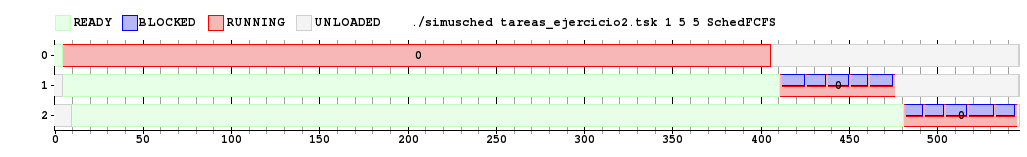
\includegraphics[width=450pt]{./figs/ejercicio2_1core.png}
\end{figure}

\begin{figure}[h]
	\centering                                                       
	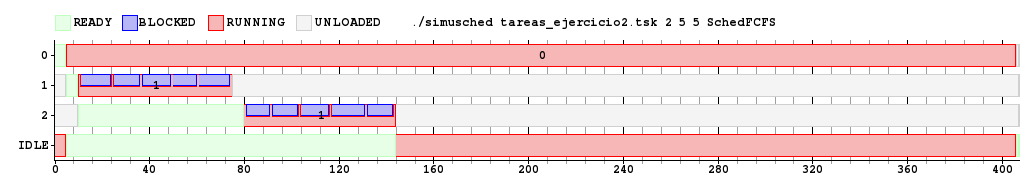
\includegraphics[width=450pt]{./figs/ejercicio2_2cores.png}
\end{figure}

\begin{figure}[h]
	\centering                                                       
	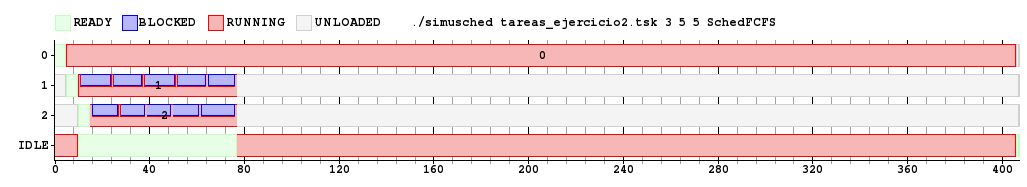
\includegraphics[width=450pt]{./figs/ejercicio2_3cores.png}
\end{figure}

Lo que se puede ver el primer gráfico es la corrida de las 3 tareas con un sólo núcleo. Estas tareas se corren de manera secuencial en el procesador y cuando termina una comienza la siguiente, siempre y cuando haya pasado el tiempo de inicio (sino es como si la misma no existiera). La primer tarea es la que usa constantemente el CPU durante un tiempo fijado (400) en el archivo del lote de tareas. Luego se ejecutan las tareas con interrupciones aleatorias (5 interrupciones con duraciones al azar entre 10 y 15ms).

En el segundo gráfico ya podemos ver cierto grado de multiprogramación, en el cual hay momentos con 2 tareas corriendo al mismo tiempo, en cada uno de los 2 cores que posee el sistema. El primer core se ocupa durante todo el tiempo de ejecución de la primera tarea, teniendo el segundo core, momentos donde ejecuta la segunda tarea, otros donde ejecuta la tercera y finalmente, tiempo idle en el que no hace nada.

En el tercer gráfico podemos ver nuevamente multiprogramación, pero esta vez con una mayor presencia de la tarea idle, ya que se corren al mismo tiempo las tareas de consola, terminando más rápido que en la simulación anterior. La tarea de CPU sigue tardando lo mismo que en los casos anteriores.

En todos los casos podemos ver el funcionamiento correcto del algoritmo FCFS, dado que las tareas se ejecutan en el mismo órden en el que llegan, como se esperaba.
\newpage

%%%%%%%%%%%%%%%%%%%%
%    Ejercicio 4    				 %
%%%%%%%%%%%%%%%%%%%%

\section{Ejercicio 4}

A continuación mostramos algunas corridas del algoritmo \textit{Round Robin}. Todas fueron ejecutadas con un lote de 5 tareas TaskCPU de 50 ticks de duración definidas en \textit{tareas\_ejercicio4.tsk}. En todas las corridas, tanto el costo de cambio de contexto como el costo de cambio de núcleo de procesamiento son iguales, para facilitar la lectura de los gráficos.

\subsection{Single-core}
\begin{figure}[h]
	\centering                                                       
	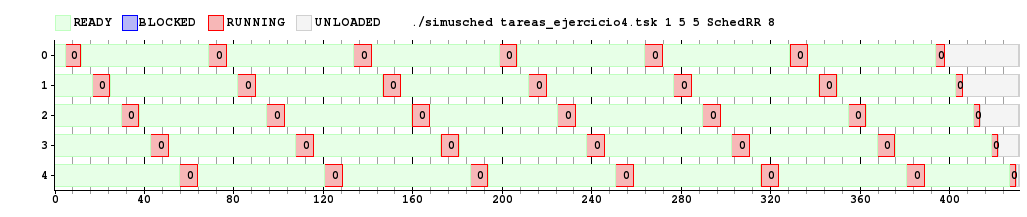
\includegraphics[width=450pt]{./figs/ejercicio4_1core.png}
\end{figure}

En esta corrida del lote se puede ver claramente el comportamiento del algoritmo \textit{Round Robin}, dado que con un quantum de 8 ticks para cada tarea, se ejecuta en el único core de prueba, alguna tarea durante ese tiempo hasta que terminan todas.

\subsection{Multi-core, igual quantum}
\begin{figure}[h]
	\centering                                                       
	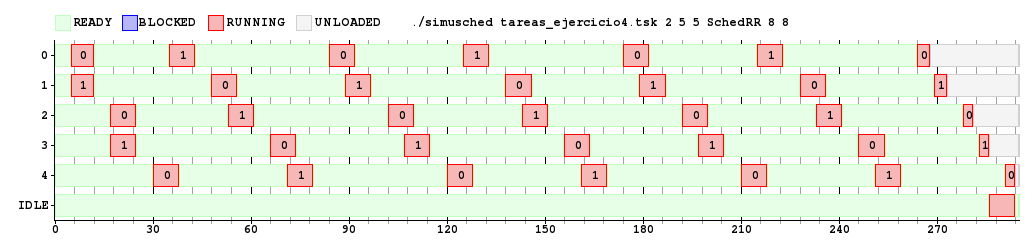
\includegraphics[width=450pt]{./figs/ejercicio4_2cores_igual_quantum.png}
\end{figure}

\begin{figure}[h]
	\centering                                                       
	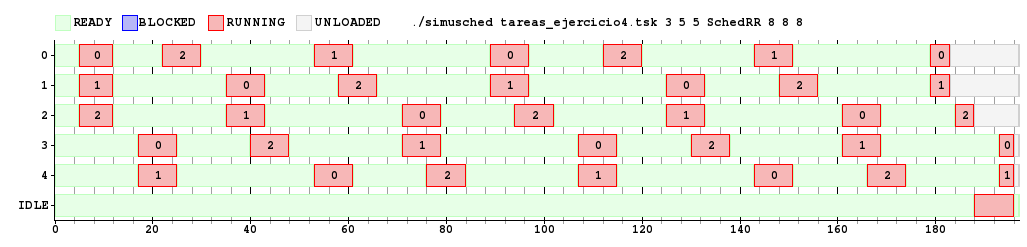
\includegraphics[width=450pt]{./figs/ejercicio4_3cores_igual_quantum.png}
\end{figure}

En estas corridas del lote se ve como se ejecutan a la vez 2 y 3 tareas durante un quantum fijo e igual para todos los núcleos. Es fácil ver como durante los primeros 2 quantums se mantiene visible el comportamiento del algoritmo. Más adelante se hace un poco más difícil de ver, pero nunca deja de apreciarse la manera secuencial característica de asignación de CPU de este algoritmo.

\clearpage

\subsection{Multi-core, distinto quantum}
\begin{figure}[h]
	\centering                                                       
	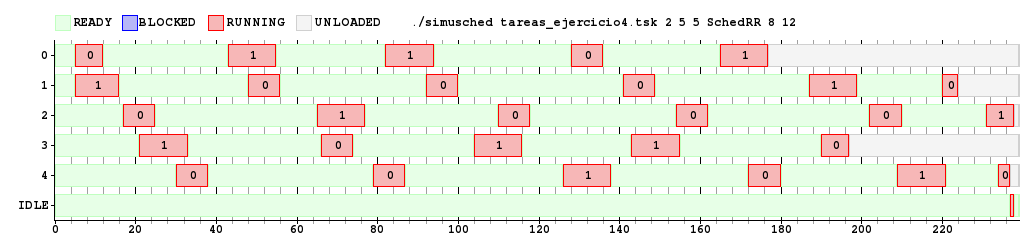
\includegraphics[width=450pt]{./figs/ejercicio4_2cores_dif_quantum.png}
\end{figure}

\begin{figure}[h]
	\centering                                                       
	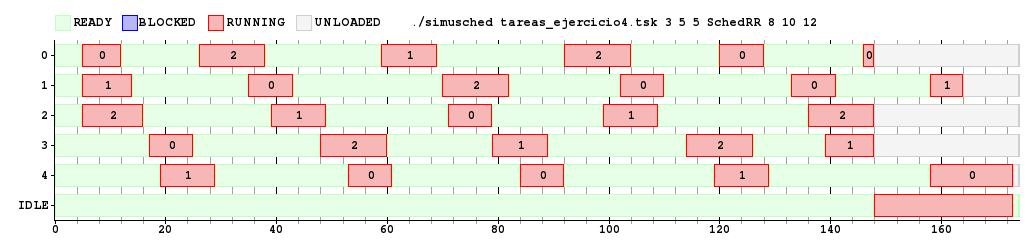
\includegraphics[width=450pt]{./figs/ejercicio4_3cores_dif_quantum.png}
\end{figure}

Estas corridas son similares a las multi-core con igual quantum. La única diferencia es el tiempo que permanece cada tarea en ejecución en alguno de los CPUs. Una misma tarea puede utilizar distinta cantidad de quantum según el core en el que se esté ejecutando. Nuevamente, se ve el comportamiento cíclico del scheduling de los procesos del algoritmo de \textit{Round Robin}.

\clearpage

\subsection{Distintas perspectivas de un mismo lote}

\begin{figure}[h]
	\centering                                                       
	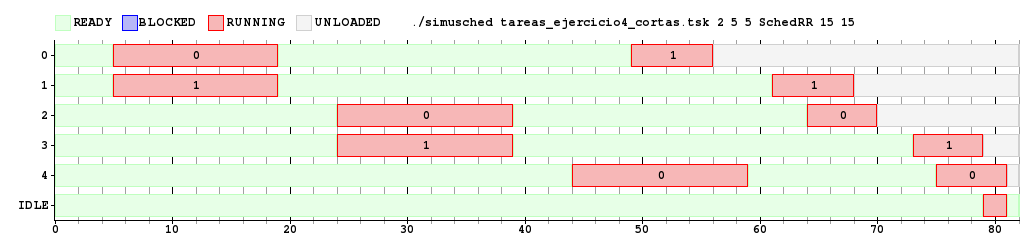
\includegraphics[width=450pt]{./figs/ejercicio4_tareas_largas.png}
\end{figure}

\begin{figure}[h]
	\centering                                                       
	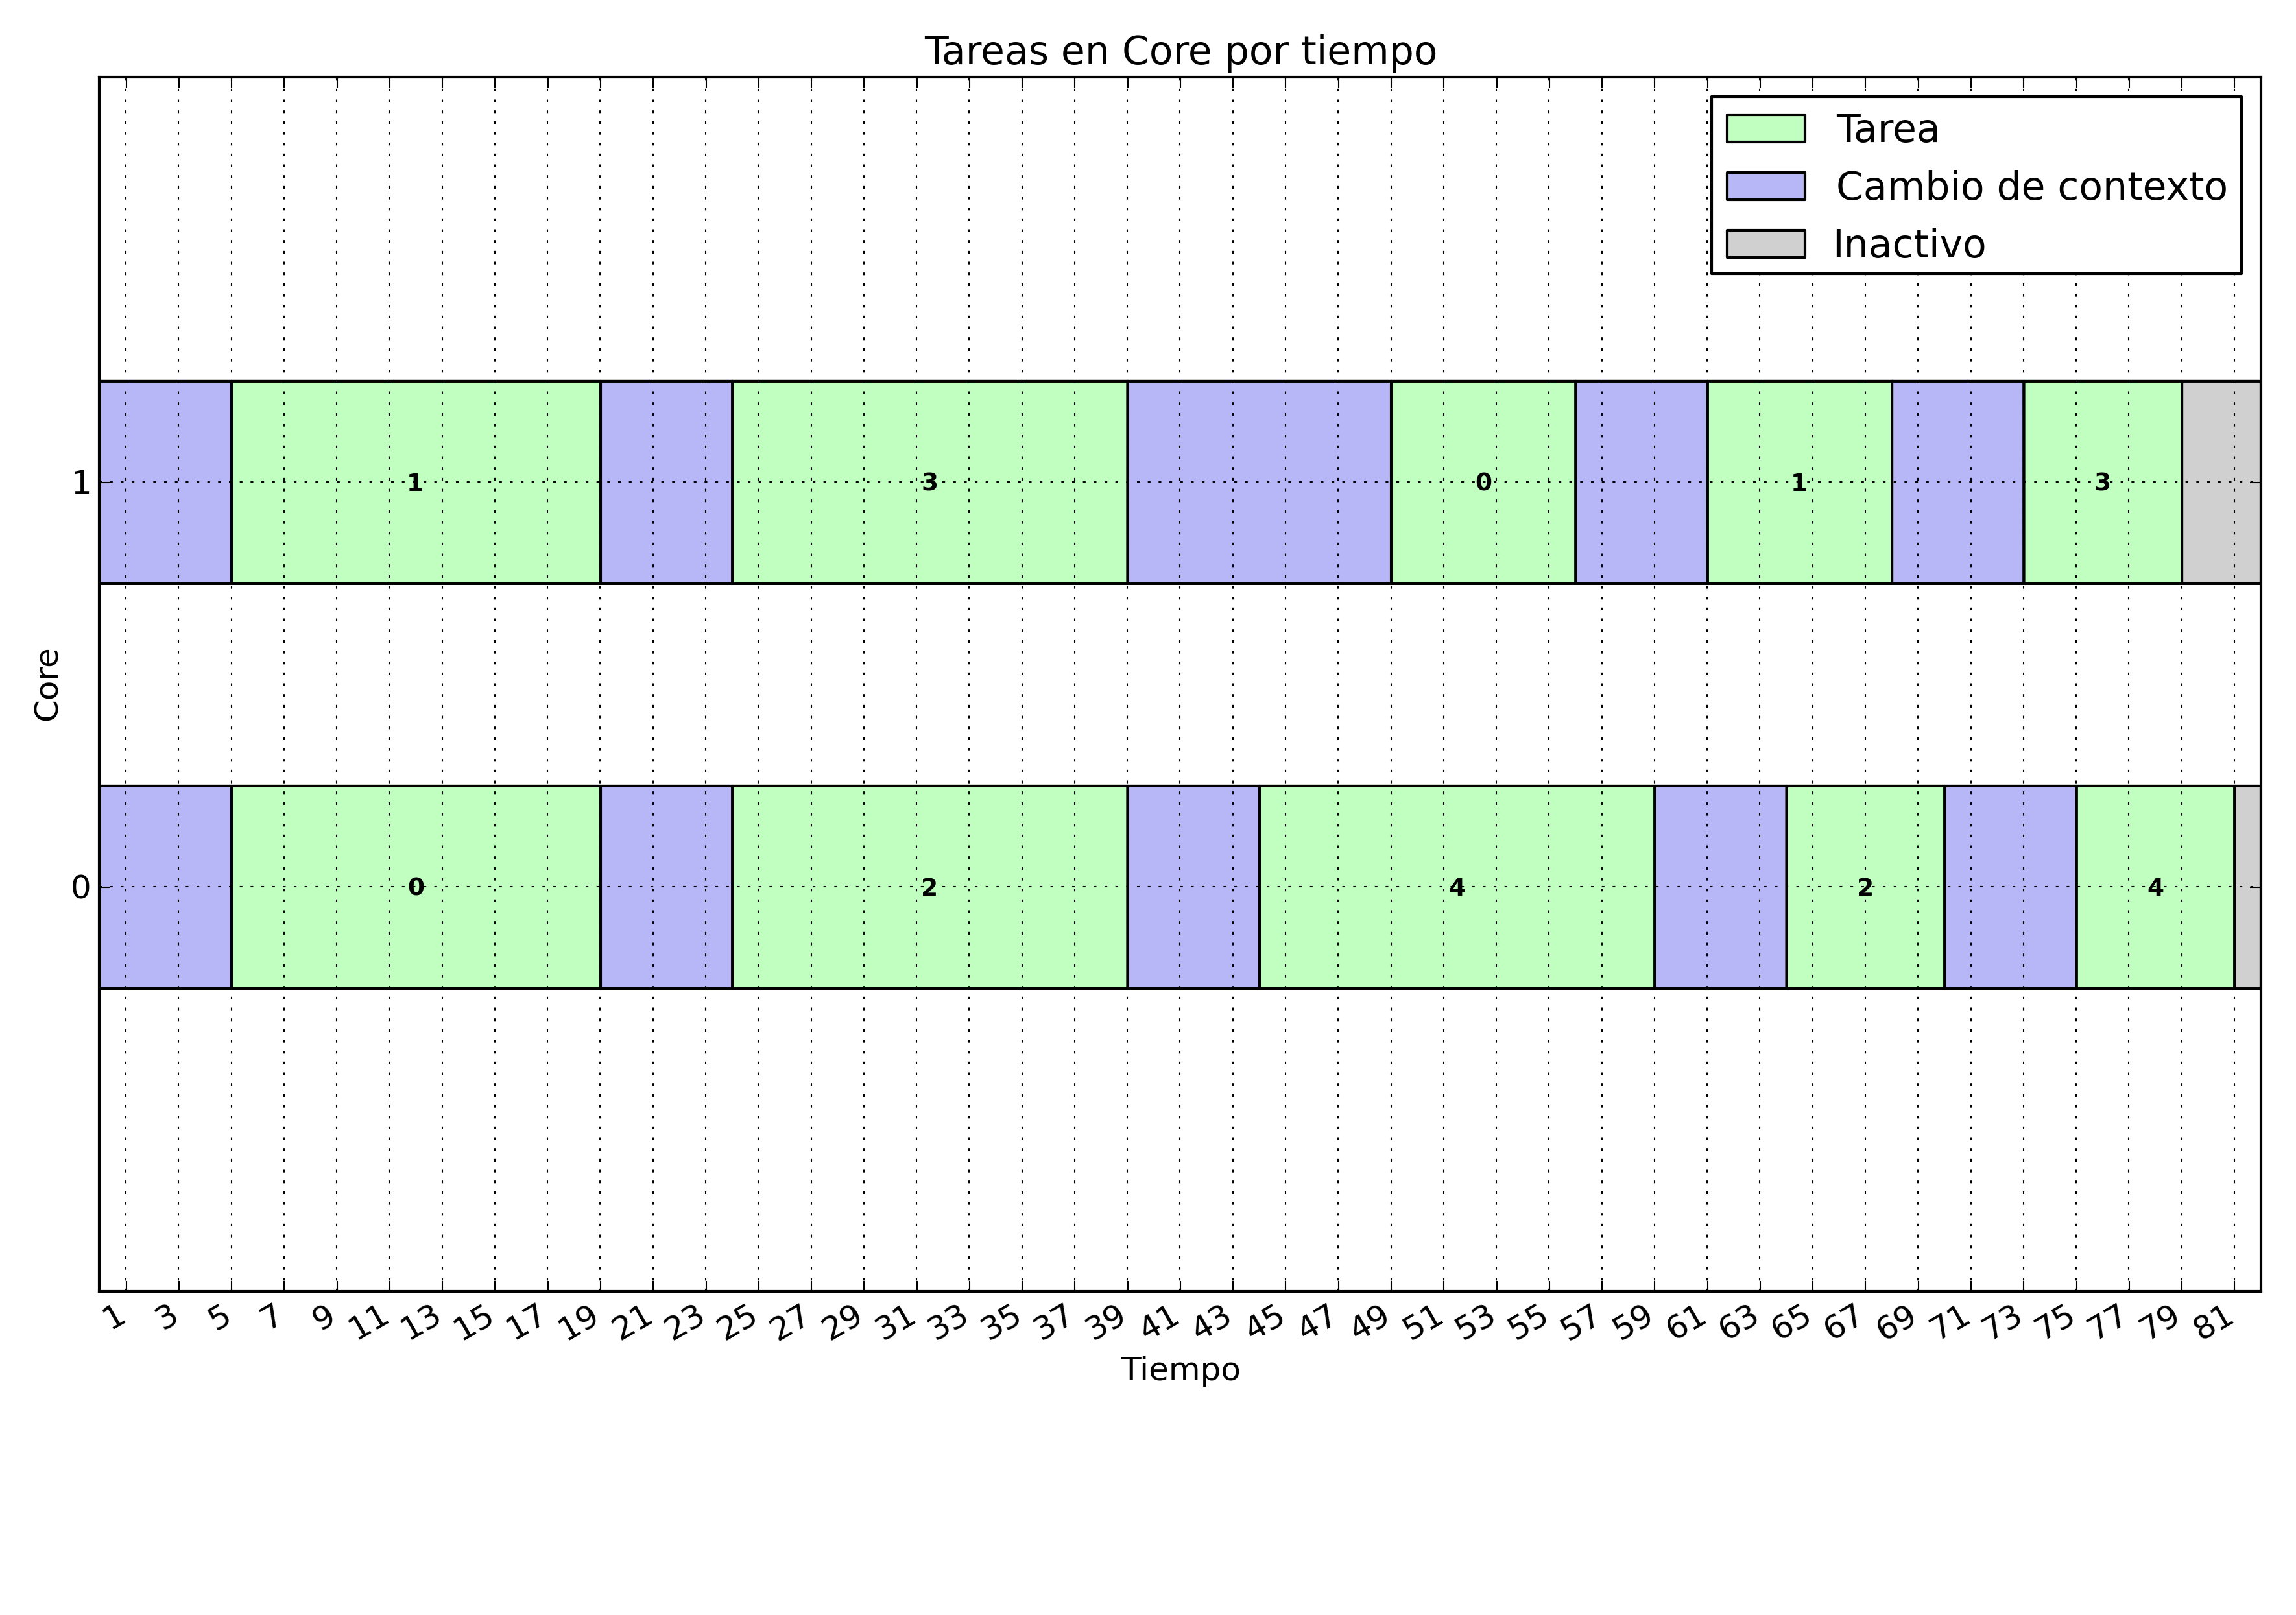
\includegraphics[width=450pt]{./figs/ejercicio4_tareas_largas_cores.png}
\end{figure}


Estos 2 gráficos son dos perspectivas diferentes de una misma corrida de un lote con 2 cores. Lo que se puede ver en el primer gráfico, es la forma en la que \textit{Round Robin} delega las tareas de manera iterativa como vimos anteriormente. En el segundo se ve la carga de cada core en un momento dado. Al ponerle el mismo quantum a ambos cores, es más fácil de ver el accionar del algoritmo.\\
\\
\indent Lo que se puede mencionar como detalle presente en estos 2 gráficos, es la forma de elegir los cores que tiene el algoritmo al finalizar su quantum por primera vez la tarea 4. Se ve claramente que, por más que al momento de ejecutarse la tarea 1 por segunda vez, el core 0 esté libre, al momento de terminar de ejecutar la tarea 0, el mismo todavía estaba siendo ocupado por la tarea 4. Por este motivo, el scheduler elige nuevamente el core 1 para trabajar, y continúa la ejecución normalmente.
\newpage

%%%%%%%%%%%%%%%%%%%%
%    Ejercicio 5  				 %
%%%%%%%%%%%%%%%%%%%%

\section{Ejercicio 5}

La implementación de $RSDL$ en este trabajo busca reflejar las características más importantes de este algoritmo dentro de un entorno y dinámica de trabajo un tanto simplificado. El resultado es un $scheduler$ que eventualmente otorga los recursos del CPU a todas las tareas (de ahí la característica de $fairness$ que se analiza más adelante y la ausencia de inanición) pero que no obstante las maneja de acuerdo a ciertos niveles de prioridad.\\
\indent La clase $SchedRSD$ cuenta con varias estructuras soporte. Por un lado utilizamos dos vectores correspondientes a las 'escaleras': uno comienza siendo el activo y es allí donde, en cada nivel, se encolan las tareas. Luego de las distintas rotaciones si no quedan más niveles para que las tareas desciendan se las introduce en la segunda escalera. Una vez que no queda ninguna tarea por ejecutar en la activa, se realiza un swap y se resume la ejecución bajo las condiciones iniciales. Adicionalmente se utilizan otros dos arreglos, uno para almacenar la cuota de tiempo asignada para los procesos en determinado nivel y otro para llevar control de la cuota global restante en cada nivel. En cuanto a la información relacionada con los procesos, se decidió utilizar dos diccionarios para guardar, en uno, los procesos bloqueados y el nivel en el que estaban al haber entrado a ese estado y, en otro, los procesos y sus cuotas individuales restantes. Finalmente, al igual que en el scheduler $Round Robin$ se cuenta con un vector de cpus y sus correspondiente arreglos de ticks transcurridos para la tarea actual y de quantum. Es importante aclarar que a diferencia de $RR$ y a pesar de conservar las mismas estructuras aquí no se utiliza el algoritmo como multicore debido a la complejidad de una implementación así.\\
\indent La inicialización del scheduler responde más que nada a cuestiones técnicas, como por ejemplo leer los parámetros y crear las estructuras de manera dinámica, llenar cada nivel con colas vacías, etc. Lo más relevante para destacar es que en principio la cuota global de cada nivel es $0$ ya que su valor estará dado por las cuotas individuales de los procesos que se carguen en cada uno. \\
\indent El siguiente paso consiste en la carga de tareas. Aquí se tomaron varias decisiones que vale la pena comentar. En lo que respecta a la prioridad inicial de una tarea no hay manera de poder determinarla al momento de carga. Tampoco creemos que asignar algún valor aleatorio fuera positivo, pues probablemente se subestimarían tareas con requerimiento de alta prioridad. La conclusión a la que llegamos fue sobreestimar a todas ellas y colocarlas en el máximo nivel de prioridad ($0$). Eventualmente aquellas tareas que se bloquean (es decir que son interactivas) no consumen su tiempo y permanecen en niveles de prioridad altos mientras el resto de las tareas comunes baja. Esto está garantizado en nuestra implementación por el hecho de que el diccionario de tareas bloqueadas recuerda el nivel donde estaba activo el proceso y porque una vez definidas allí las tareas no consumen su cuota ni participan de la rotación de cada nivel. Luego, a la primera tarea cargada se le asigna el cpu mientras que el resto se encolan en el nivel de prioridad correspondiente. Al realizar esta función también reflexionamos sobre qué debería suceder si una tarea fuera cargada en medio de la simulación. A diferencia de un desbloqueo, donde se acentúa y preserva la prioridad de tareas interactivas, una tarea completamente nueva no debería poder ser cargada en un nivel de mayor prioridad al activo en ese momento. Esto podría impactar negativamente en la fluidez y desarrollo del scheduler dado que si hubiera pasado un tiempo considerable y todas las tareas hubieran bajado hasta uno de los últimos peldaños de la escalera, la repentina llegada de una tarea a un nivel alto implicaría un retraso importante en el resto. Luego, decidimos que la prioridad de nuevas tareas durante la ejecución fuera la del nivel activo.\\
\indent Por último resta hablar de la función $tick()$, la cual se encarga del grueso de la lógica de esta técnica de scheduling. A grandes rasgos el mecanismo permanece igual que en el resto de los schedulers: tenemos los tres motivos posibles y en cada uno el comportamiento particular para cada tarea es el mismo: o la tarea termina, o se bloquea, o ejecuta normalmente. En cualquier caso el scheduler debe determinar qué tarea devolver como siguiente y qué hacer con la tarea actual, y es aquí donde aparecen las ideas particulares de $RSDL$. Dependiendo del estado de la cuota del nivel actual, del proceso que está corriendo o del quantum restante habrá muchas maneras de proceder: para el motivo tick, puede que el proceso siga ejecutándose o que su cuota individual haya expirado y deba cambiárselo de nivel. También puede suceder que la cuota global del nivel se haya agotado (debido a nuestra implementación eso necesariamente se superpondrá con el agotamiento del proceso actual, dado que la cuota global es la suma de las cuotas de los procesos corriendo) en cuyo caso se realiza una rotación menor (la cola de procesos se baja de nivel). En caso de que no quedaran más niveles se realiza una rotación mayor, que en el caso de esta implementación implica realizar un swap entre los punteros asignados a ambas escaleras puesto que los procesos ya deberían haber sido encolados en los lugares correspondientes.

\newpage

%%%%%%%%%%%%%%%%%%%
%    Ejercicio 7    			   %
%%%%%%%%%%%%%%%%%%%

\section{Ejercicio 7}

%\subsection{Conclusiones preliminares}
%\begin{itemize}
%	\item Para todos los experimentos existe un quantum a partir del cual aumentarlo no cambia la performance del sistema.
%	\item Para la métrica CPU utilization (que mide la cantidad de tiempo que el CPU está ocupado, entre 0 y 100\% del tiempo, queriendo tenerlo el mayor tiempo ocupado posible), se puede ver con 1 core, que cuando las tareas tienen distinta cantidad de llamadas bloqueantes, el uso del CPU es muy alto, casi 100\%, siendo los ticks de exit de cada tarea al terminar, los únicos que se desperdician. Es decir, se utiliza el CPU durante \textit{cantidad\_total\_de\_ticks - cantidad\_de\_tareas}. Se ve en \textit{ejercicio7\_1core\_quantumX.png} y se estabiliza a partir del test que tiene quantum 8.
%\end{itemize}

Para la resolución de este ejercicio debimos elegir al menos 2 métricas para evaluar la performance de nuestro algoritmo \textit{Round Robin}. A continuación, nuestra experimentación y sus resultados.

\subsection{CPU Utilization}

Para evaluar la performance de nuestro algoritmo con la métrica de utilización del CPU hicimos tanto pruebas single-core como pruebas multi-core, pero lo que queremos mostrar se ve de manera más clara en las pruebas single-core. Los experimentos fueron los siguientes:

\begin{figure}[h]
	\centering                                                       
	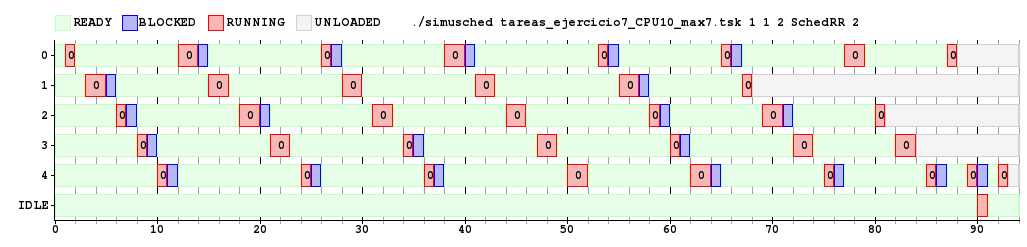
\includegraphics[width=450pt]{./figs/ejercicio7_1core_quantum2.png}
\end{figure}

En la primera prueba, con un quantum de 2 ticks para cada core, podemos ver que la utilización del único CPU disponible es durante un tiempo considerable (poco más de 83\%, siendo lo normal entre 40 y 90\% en un escenario real\footnote{Operating System Concepts - 7th Edition - página 157}).

\begin{figure}[h]
	\centering                                                       
	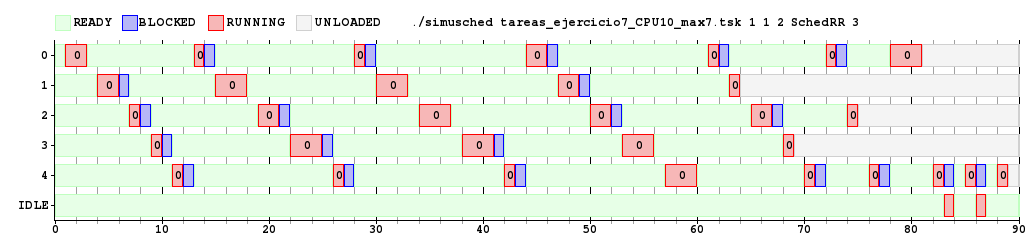
\includegraphics[width=450pt]{./figs/ejercicio7_1core_quantum3.png}
\end{figure}

Aumentando levemente el quantum a 3 ticks por turno, se ve que el \textit{turnaround time}, del cual hablaremos en breve, disminuye, y también el uso del CPU mejora, teniendo menos momentos de CPU en estado ocioso (86$\sim$87\% de tiempo de CPU ocupado).

\begin{figure}[h]
	\centering                                                       
	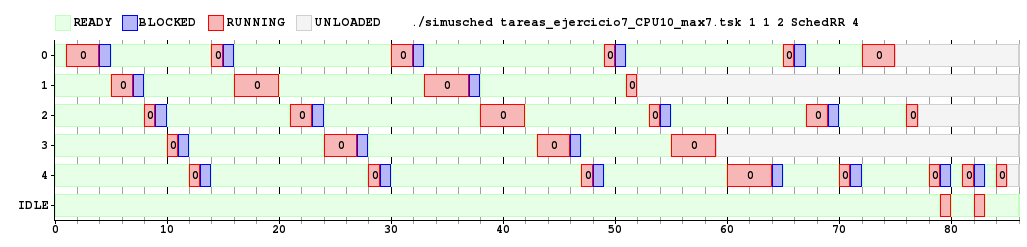
\includegraphics[width=450pt]{./figs/ejercicio7_1core_quantum4.png}
\end{figure}

Con un quantum de 4 ticks, el rendimiento del CPU llega a un 90$\sim$91\%, disminuyendo otra vez el \textit{turnaround time}, pero aumentando el quantum todavía se puede mejorar, como veremos a continuación.

\clearpage

\begin{figure}[h]
	\centering                                                       
	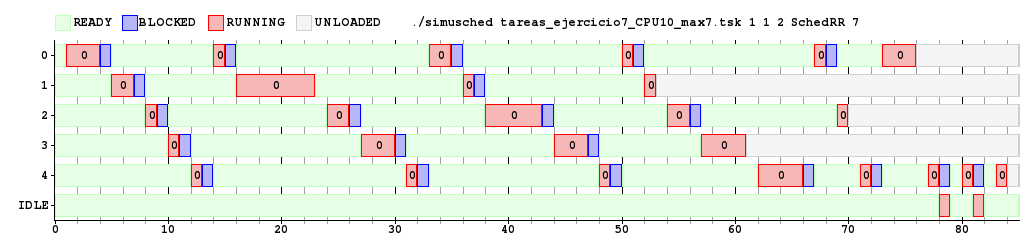
\includegraphics[width=450pt]{./figs/ejercicio7_1core_quantum7.png}
\end{figure}

\begin{figure}[h]
	\centering                                                       
	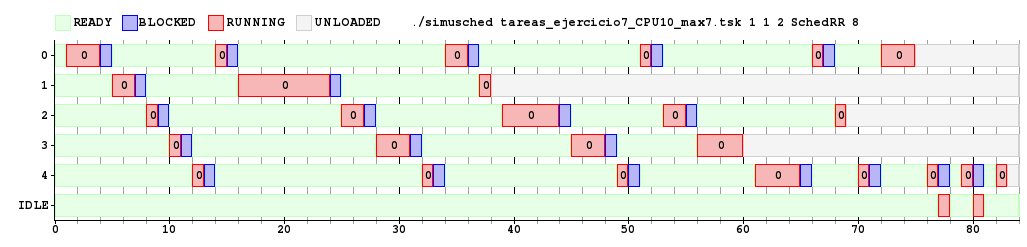
\includegraphics[width=450pt]{./figs/ejercicio7_1core_quantum8.png}
\end{figure}

\begin{figure}[h]
	\centering                                                       
	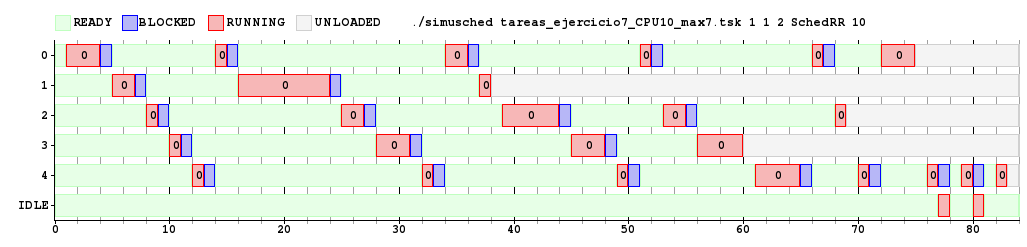
\includegraphics[width=450pt]{./figs/ejercicio7_1core_quantum10.png}
\end{figure}

Hasta un quantum de 7 ticks inclusive, la tarea 1 debe consumir al menos 4 quantums para completarse. A partir de los 8 ticks, en 3 quantums la misma completa su ejecución y termina, disminuyendo drásticamente su \textit{turnaround time}, dado que su \textit{waiting time} se recorta en un turno completo. En el sistema en general, el aumentar el quantum más allá de los 8 ticks por turno ya no mejora la performance del mismo.

\clearpage

\textbf{Perspectiva del core: quantum = 2:}
\begin{figure}[h]
	\centering                                                       
	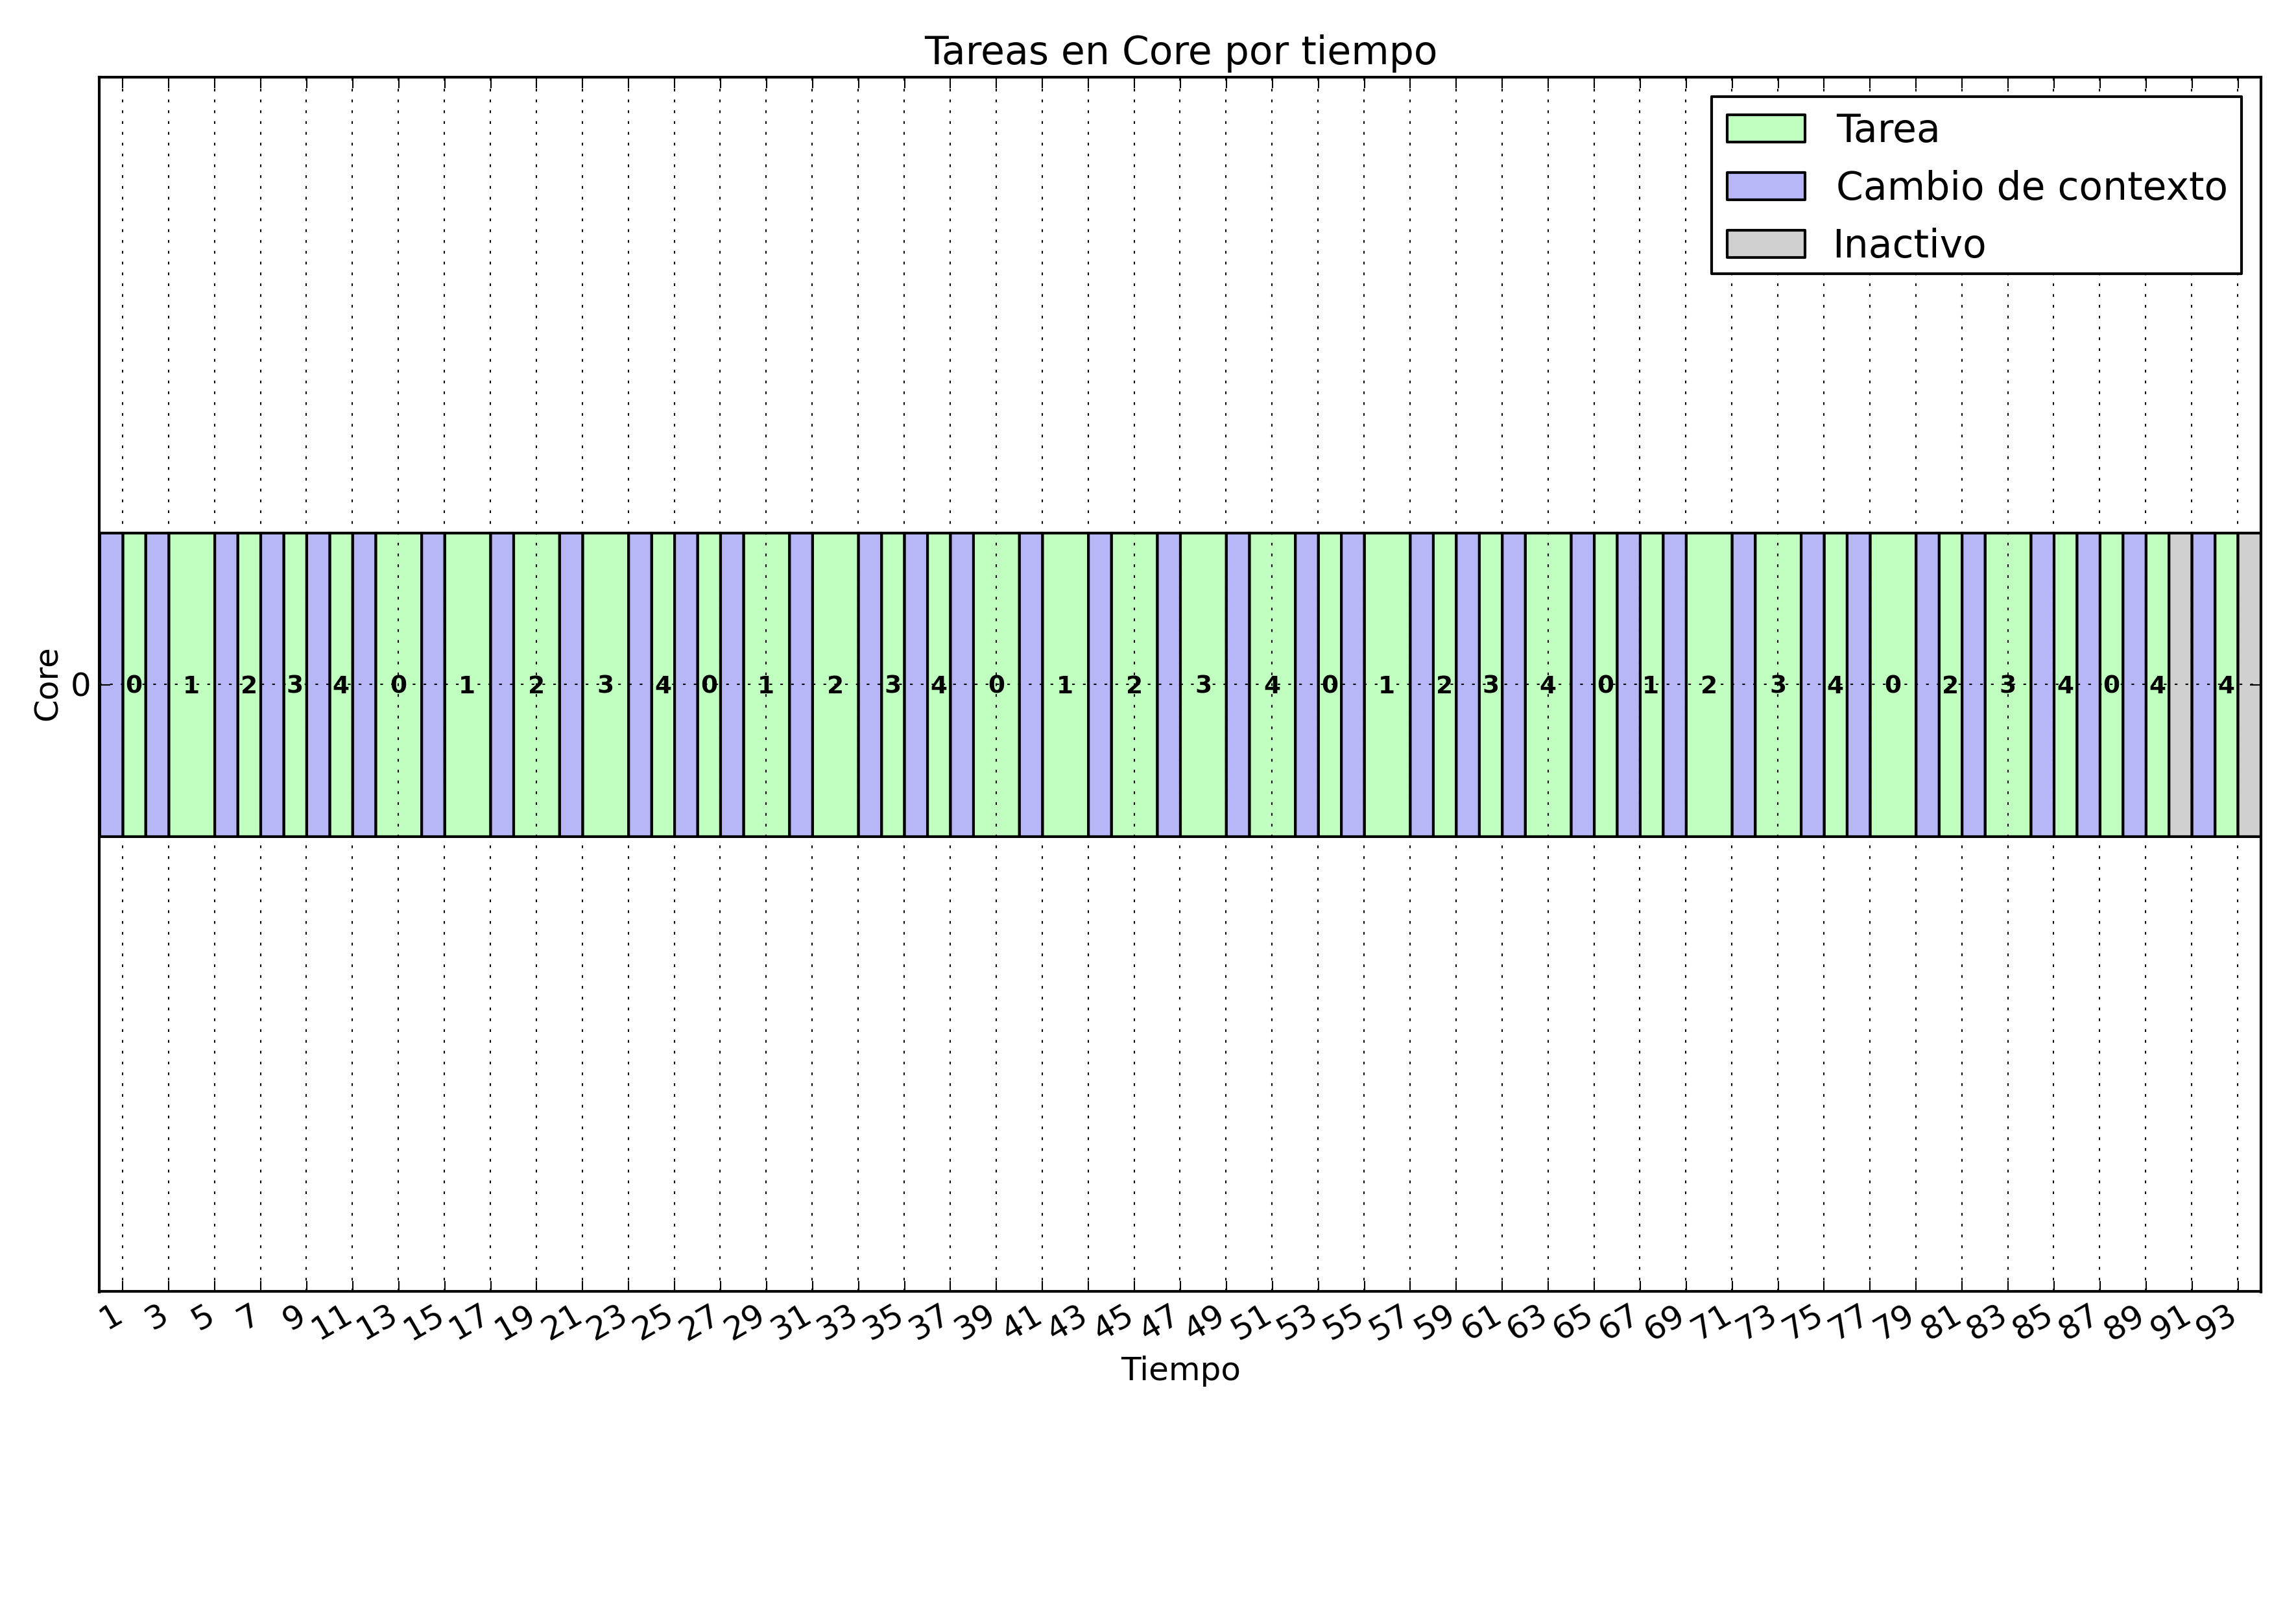
\includegraphics[width=350pt]{./figs/ejercicio7_cores_quantum2.png}
\end{figure}

\textbf{Perspectiva del core: quantum = 10:}
\begin{figure}[h]
	\centering                                                       
	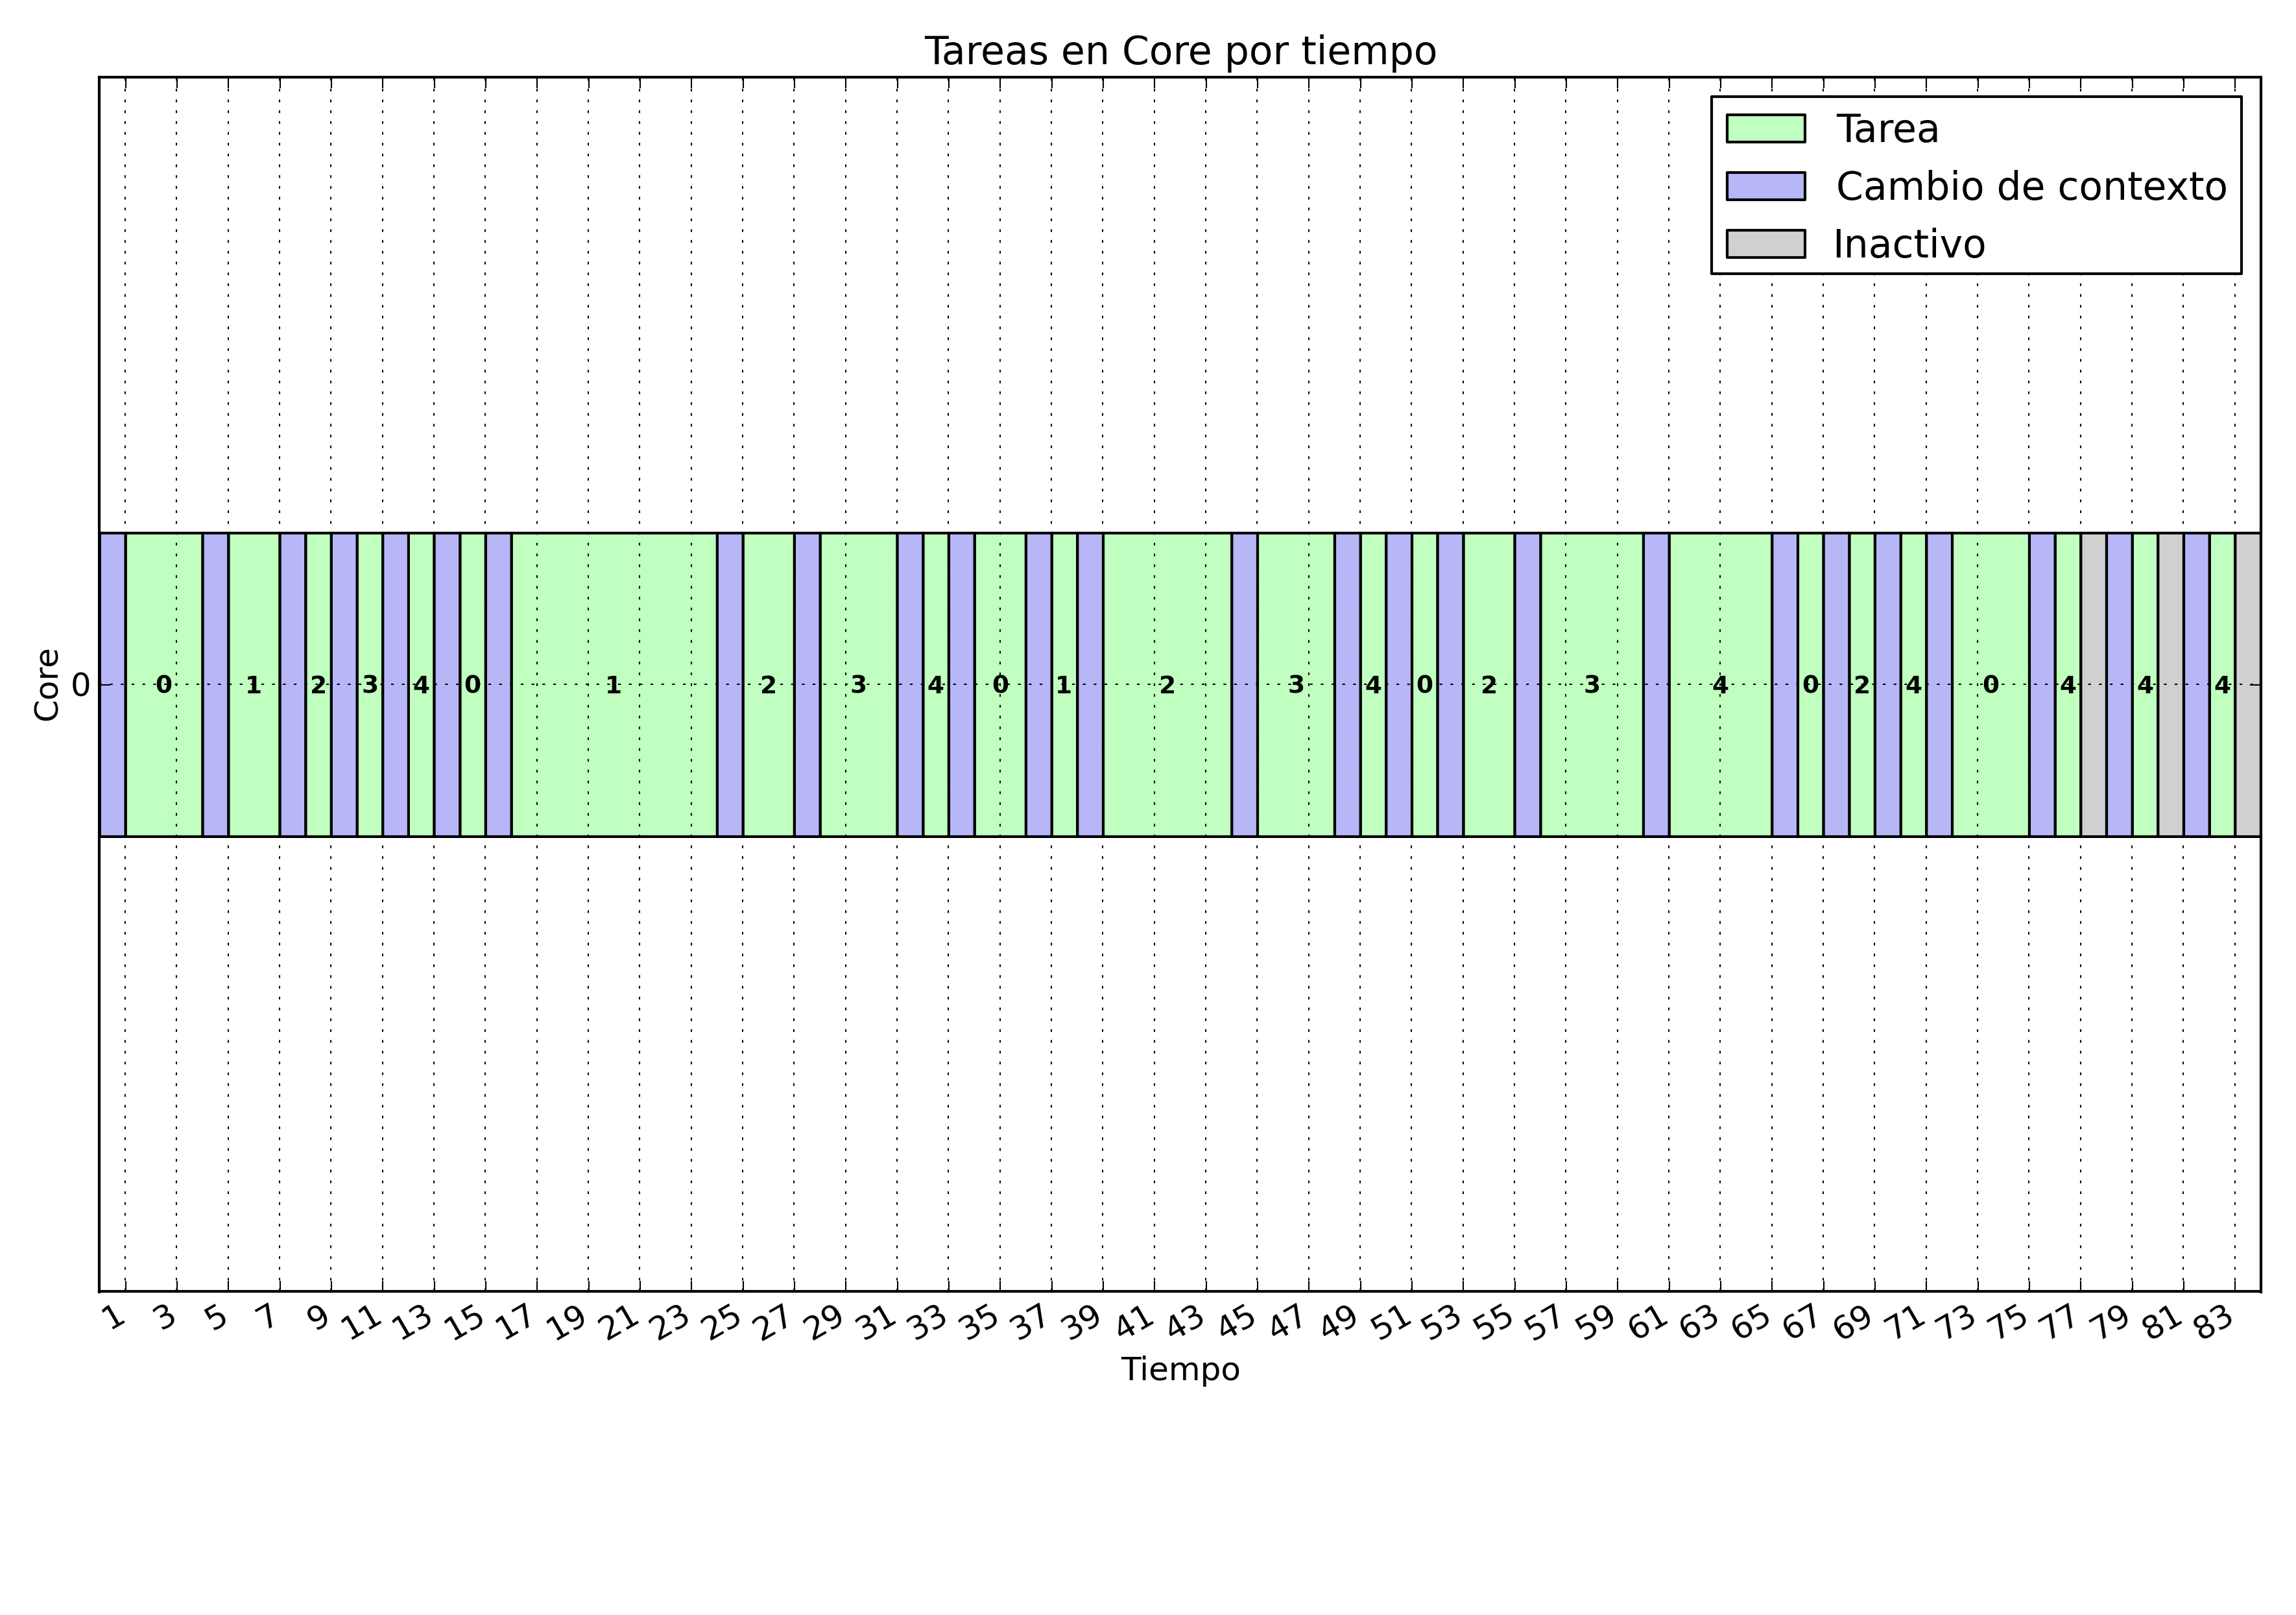
\includegraphics[width=350pt]{./figs/ejercicio7_cores_quantum10.png}
\end{figure}

Para terminar el análisis de este criterio, podemos concluir que el quantum óptimo para este experimento es 8 ticks, y como comentario agregado, podemos decir que se nota la importancia de una buena elección del quantum, viendo que entre el uso de CPU con quantum 2 y el uso con quantum 8, hay una mejora de un 10.63\% aproximadamente.

\subsection{Turnaround time y Waiting time}

Decidimos evaluar el desempeño del algoritmo con los criterios de \textit{turnaround time} y \textit{waiting time} de manera conjunta, ya que creemos que en este tipo de experimentos están íntimamente ligados, al menos en este escenario de prueba. Esto es porque las tareas no son interactivas, en cuyo caso habría que ver también (y por separado) el \textit{response time}, que se encarga de evaluar el tiempo neto utilizado por el CPU una vez que se terminó la interacción con el usuario\footnote{Operating System Concepts - 7th Edition - página 157, 158}, que en general, es órdenes de magnitud más lento que lo que vimos hasta ahora.\\

\textbf{2 cores:}
\begin{figure}[h]
	\centering                                                       
	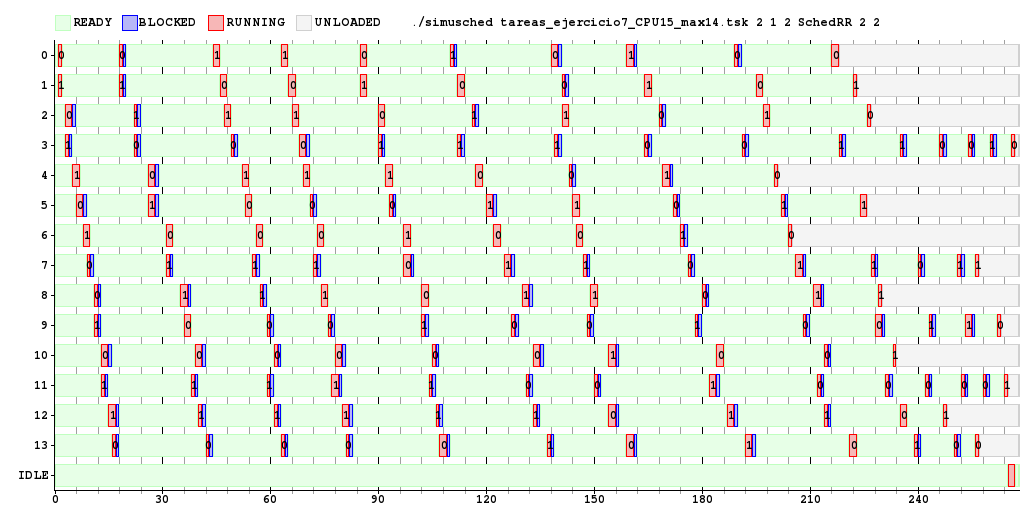
\includegraphics[width=450pt]{./figs/ejercicio7_t15_2cores_quantum2.png}
\end{figure}

\begin{figure}[h]
	\centering                                                       
	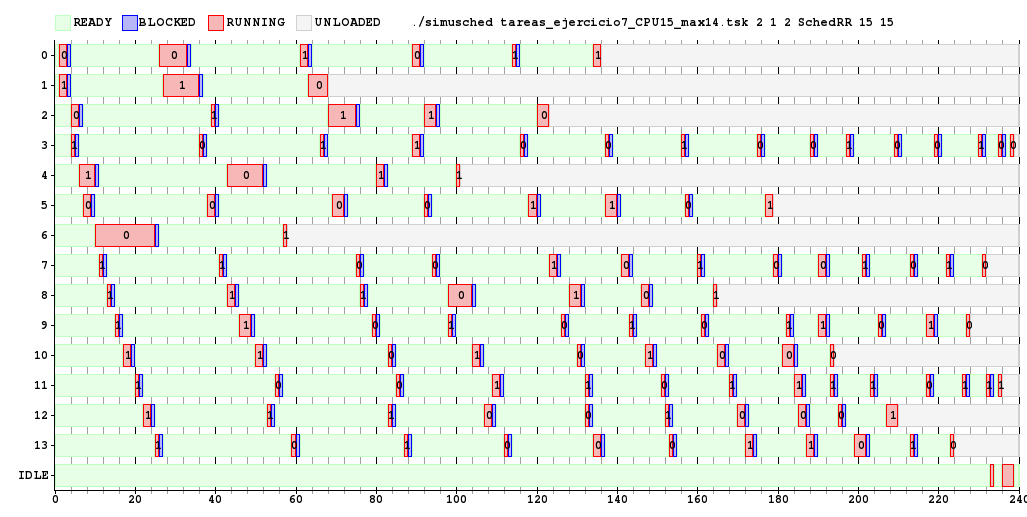
\includegraphics[width=450pt]{./figs/ejercicio7_t15_2cores_quantum15.png}
\end{figure}

En el ejemplo con 2 núcleos se puede ver una mejora sustancial entre un quantum pequeño (2 ticks) y que corta muchas veces la ejecución de cada tarea, contra el quantum óptimo (15 ticks) que interrumpe menos veces la ejecución. Dicha mejora es de alrededor de 24 ticks, o aproximadamente un 10\% menos en el \textit{turnaround time}.\\
\indent Además se puede apreciar como en la mayoría de las tareas, el \textit{waiting time} es drásticamente reducido gracias al aumento del quantum por turno, teniendo hasta 7 turnos menos que ejecutar en casos como la tarea 1 o la 6, reduciendo el \textit{waiting time} de las tareas de manera altamente sustancial, hasta más de 120 ticks en algunos casos como por ejemplo en la tarea 6.

\clearpage

\textbf{3 cores:}
\begin{figure}[h]
	\centering                                                       
	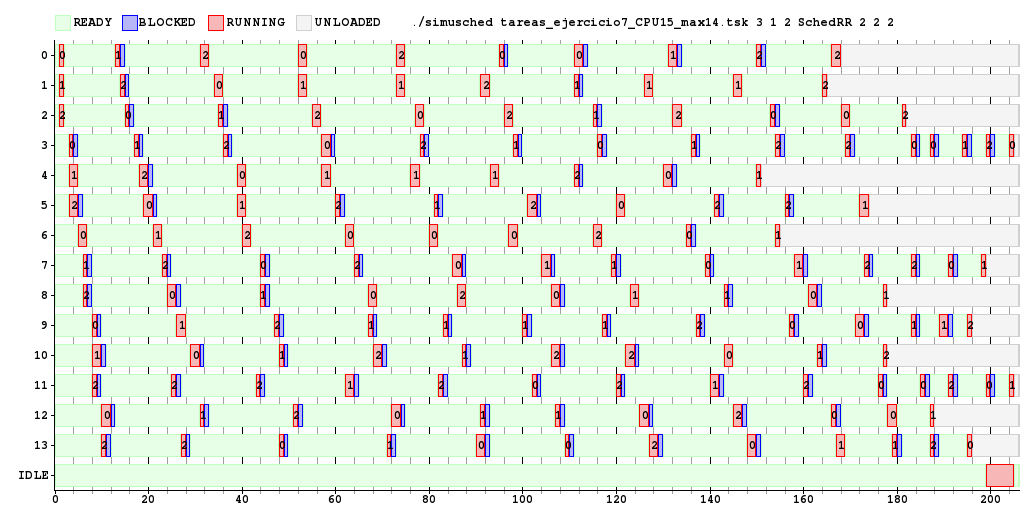
\includegraphics[width=450pt]{./figs/ejercicio7_t15_3cores_quantum2.png}
\end{figure}

\begin{figure}[h]
	\centering                                                       
	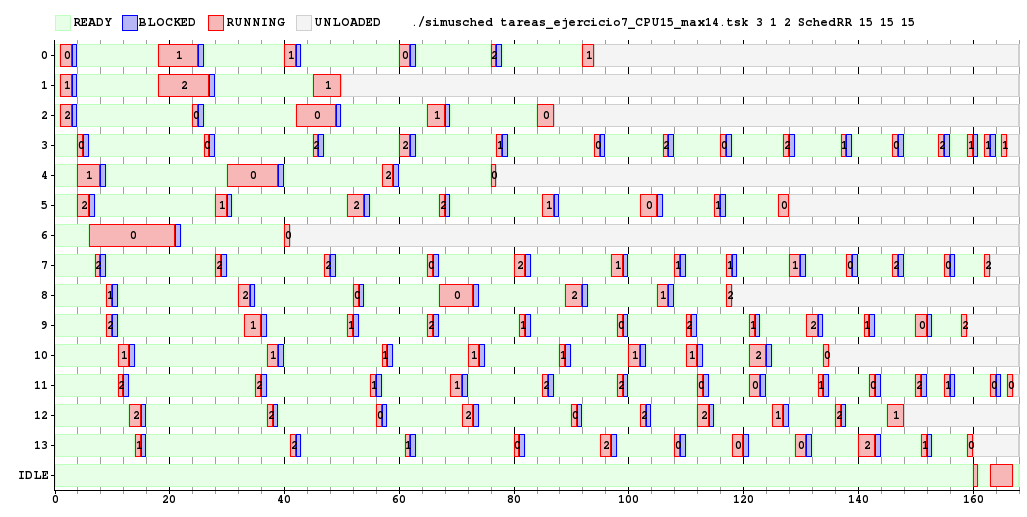
\includegraphics[width=450pt]{./figs/ejercicio7_t15_3cores_quantum15.png}
\end{figure}

\clearpage

\textbf{4 cores:}
\begin{figure}[h]
	\centering                                                       
	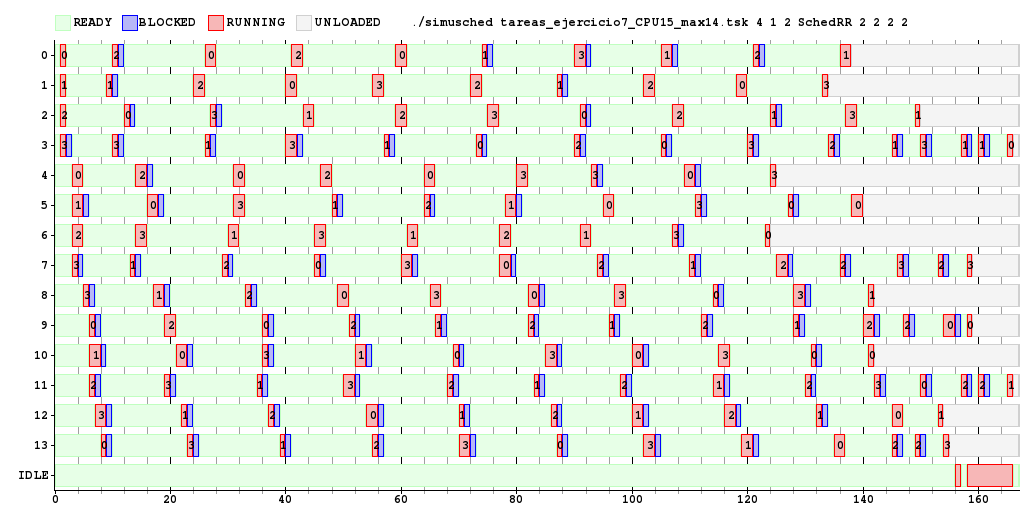
\includegraphics[width=450pt]{./figs/ejercicio7_t15_4cores_quantum2.png}
\end{figure}

\begin{figure}[h]
	\centering                                                       
	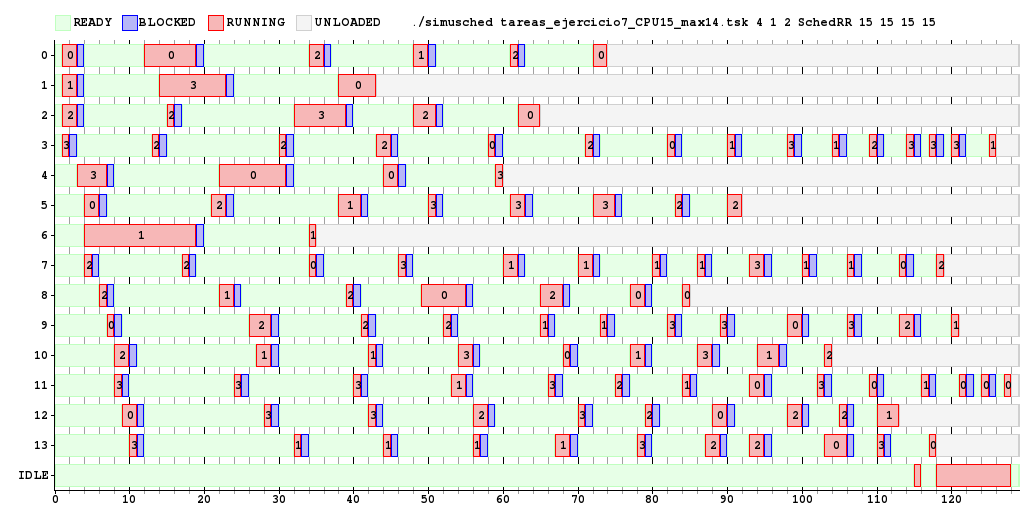
\includegraphics[width=450pt]{./figs/ejercicio7_t15_4cores_quantum15.png}
\end{figure}

Estos comportamientos se ven reflejados de manera similar en los casos con más cores (en este caso mostramos los casos de 3 y 4 cores), siendo la disminución del \textit{waiting time} proporcional a la disminución del \textit{turnaround time} total, gracias al aumento de \textit{throughput} (cantidad de tareas finalizadas en una unidad de tiempo\footnote{Operating System Concepts - 7th Edition - página 157}) debido al agregado de cores de trabajo.
\newpage

%%%%%%%%%%%%%%%%%%%%%%
%    Ejercicio 8   				 %
%%%%%%%%%%%%%%%%%%%%%%

\section{Ejercicio 8}

\subsection{Implementación de Round Robin 2}

\indent Como nos indicaba la consigna de este ejercicio, se implementó un algoritmo Round Robin que no permite migración.\\
\indent A la hora de implementarlo, nos valimos de varias estructuras de datos que nos permitiesen de alguna manera hacer un seguimiento de la tareas, para saber cual será la próxima a ejecutarse.\\
\indent Una cola de tareas llamada $procesos$, donde encolamos las tareas que todavía no tienen un core asignado. Un vector de colas llamado $colas$, de tamaño igual a la cantidad de cores. En la posición $i$ de dicho vector encontramos la cola de tareas que fueron asignadas al core $i$. El vector $cores$ , de tamaño igual a la cantidad de cores del sistema. En la posicion $i$ de $cores$ se encuentra el pid de la tarea que está corriendo actualmente en el core $i$.\\
\indent Además, tenemos el diccionario $blockedProc$, donde guardaremos el core asignado a una tarea bloqueada.\\

\indent Cuando se carga una tarea, se la asigna al primer core libre que encuentre y se la agrega a su correspondiente cola. Si estuviesen todos ocupados, se la manda a la cola $procesos$.\\
\indent Siempre que un core deba realizar un cambio de tarea, ya sea porque la que estaba corriendo consumió su quantum, o porque se bloqueó o porque finalizó, se prioriza a las tareas que todavía no fueron asignadas a algún core por sobre las que tiene dicho core asignado. Esto es porque según nuestra implementación, si una tarea está en la cola de un core entonces fue corrida por lo menos una vez en ese core y además no está en la cola $procesos$.\\
\indent Si se encontrase un elemento en $procesos$ se la saca dicha cola y se la agrega a la cola del cpu correspondiente de manera tal que sea la próxima en salir en ser desencolada.Si no hubiese más elementos en $procesos$ entonces se prosigue con la siguiente tarea de la cola y dependiendo de si se terminó el quantum de la tarea que había estado corriendo en ese tick, se la encola al final de la cola correspondiente a su core, o se simplemente se la saca de allí.\\
\indent Si una tarea se bloquease, se la define en el diccionario con su correpondiente core de clave y se la quita de la cola de ese core. Cuando se desbloquee, se obtiene el core que tiene asignado del diccionario y la borra del diccionario.\\
\indent Una vez definidas todas las tareas en cada core, el funcionamiento del algoritmo es similar a pensar un round robin común y corriente para cada core.\\


\subsection{Experimentación}

\indent Se experimentó principalmente con el siguiente lote de tareas:\\


\indent TaskBatch 10 5\\


\indent TaskBatch 10 2\\


\indent TaskBatch 10 4\\


\indent TaskBatch 10 3\\


\indent TaskBatch 10 7\\

\indent Se estudiaron casos de uno, dos y tres cores. Para los casos multicore, se analizó qué ocurría cuando todos los cores tenían valores de quantum iguales y luego, algunos casos con distintos valores de quantum para cada core.\\

\indent Una primera hipótesis que se conjeturó antes de experimentar fue que mientras más cores hubiese más rápido se terminarían de ejecutar todas las tareas. Además, intuitivamente pensamos que a partir de cierto valor de quantum no habría diferencia en ni en la forma ni el tiempo de ejecución de la tareas.\\
\indent Es importante destacar que el valor de los quantum seguramente impacte en el core al que será asignado una tarea, puesto que puede ocurrir que con un quantum chico una tarea deje de correr y el cpu agarre otra sin core asignado, mientras que con un quantum más grande quizá la tarea se hubiera quedado ejecutando y no se asignara esa nueva tarea al core.\\
\indent Además, hay que destacar que si bien el algoritmo Round Robin 2 se ahorra de alguna manera pagar los costos de migración, podría ocurrir también que al no permitir migrar tareas de core, un core tenga muchas tareas asignadas mientras que otros están vacíos (ya sea porque las que corría se terminaron o están bloqueadas), y lo lógico sería usar dicho core para ejecutar otra tarea.\\
\indent Queremos observar que existe un cierto valor de quantum para cada core a partir del cual ya no se mejora el tiempo de ejecución de todas las tareas, aunque es de notar que dicho valor también dependerá del lote de tareas a correr.\\

\subsubsection{Un Core}

\indent Lo más destacable del estudio de este caso es que se comporta igual que un Round Robin común y corriente (y es lo esperable).\\
\indent Las conclusiones de la consigna anterior valen entonces para este caso. Para ello, se provee el gráfico con un quantum igual a ocho, que es el valor de quantum donde se estabilizaba el Round Robin con un core:\\

\begin{figure}[h]
	\centering                                                       
	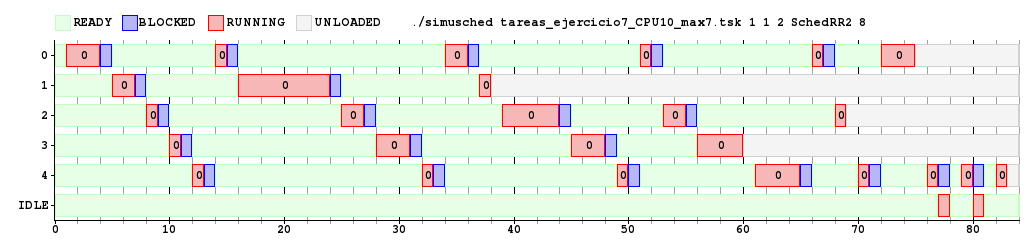
\includegraphics[width=450pt]{./figs/ej8/ej8-q8.png}
\end{figure}

\subsubsection{Dos Cores}

\indent Analicemos primero cuando ambos cores tiene el mismo quantum. Se estudiaron casos con quantums desde dos hasta diez. A partir de ellos se analizó el turnaround time y el waiting time de cada tarea.\\
\indent Veamos algunos gráficos que nos parecen sirven para ejemplificar:

\begin{figure}[h]
	\centering                                                       
	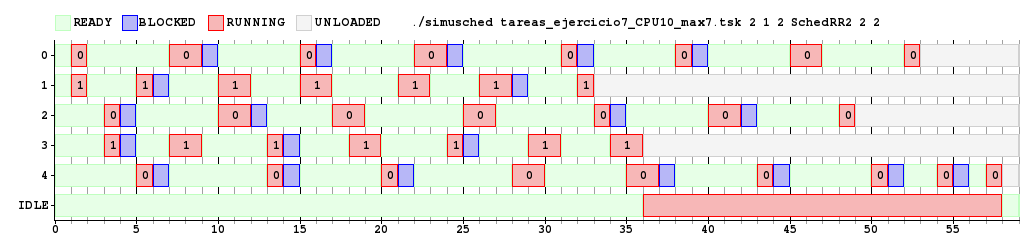
\includegraphics[width=450pt]{./figs/ej8/ej8-c2-q2.png}
\end{figure}


\begin{figure}[h]
	\centering                                                       
	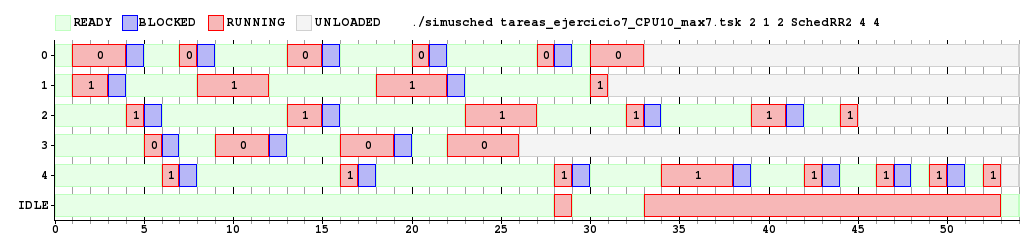
\includegraphics[width=450pt]{./figs/ej8/ej8-c2-q4.png}
\end{figure}


\indent Entre estos dos gráficos se observa como cambiando los quantum de 2 a 4 el cpu asigna las tareas de manera distinta. Se puede observar como en el primer caso la tarea 2 se ejecuta en el core 0 y en el segundo caso se ejecuta en el core 1. Algo similar ocurre con las tareas 3 y 4. Además, se observa como se terminan de ejecutar todas las tareas más rápido en este último caso.\\

\begin{figure}[h]
	\centering                                                       
	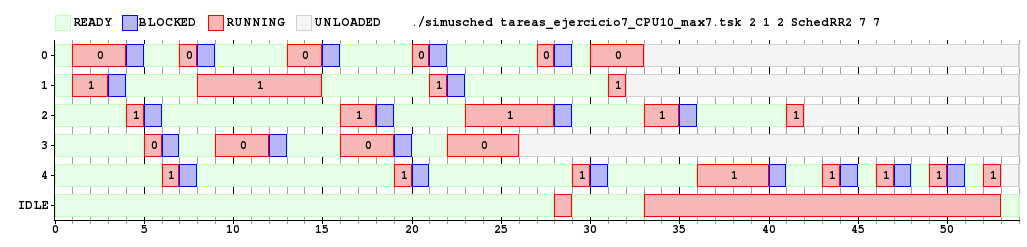
\includegraphics[width=450pt]{./figs/ej8/ej8-c2-q7.png}
\end{figure}

\begin{figure}[h]
	\centering                                                       
	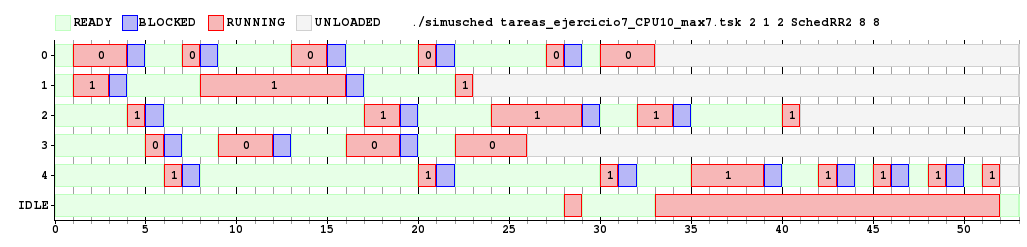
\includegraphics[width=450pt]{./figs/ej8/ej8-c2-q8.png}
\end{figure}

\begin{figure}[h]
\centering                                                       
	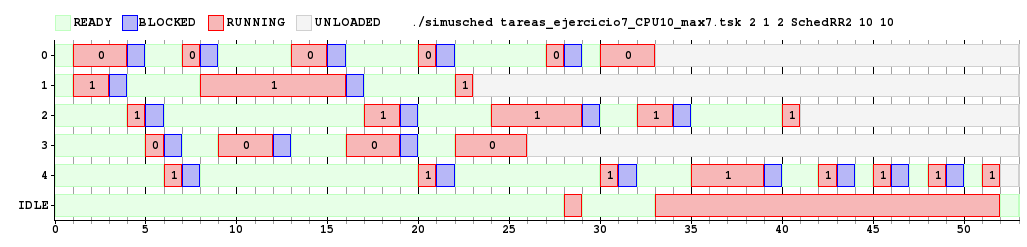
\includegraphics[width=450pt]{./figs/ej8/ej8-c2-q10.png}
\end{figure}

\indent Como ocurría en el caso de un core, observamos como a partir del caso con quantum igual a ocho, el scheduler actúa de la misma manera. Además en estos casos se observa como terminan de ejecutar todas las tareas más rápido que con quantum igual a cuatro.\\

\indent A partir de todos los casos de este tipo estudiados, se produjeron los siguientes gráficos que muestran la evolución del turnaround time y el waiting time de cada tarea en función del quantum utilizado:\\
\clearpage

\begin{figure}[h]
	\centering                                                       
	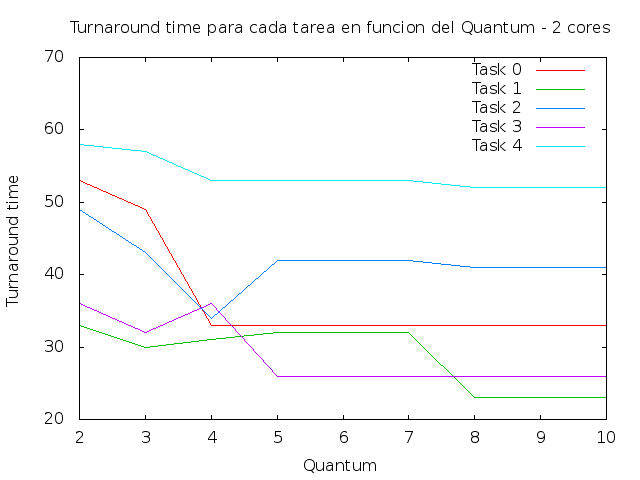
\includegraphics[width=280pt]{./figs/ej8/turnaroundtime2cores.png}
\end{figure}

\begin{figure}[h]
	\centering                                                       
	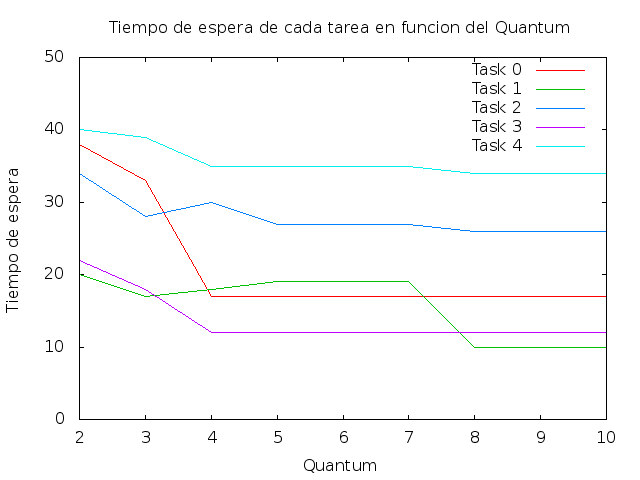
\includegraphics[width=280pt]{./figs/ej8/waitingTime2cores.png}
\end{figure}


\indent En tales gráficos se observa como en general el waiting time parece evolucionar de manera decreciente, a pesar de algunas pequeñas subidas en el gráfico hasta que se estabiliza para todas las tareas para un quantum igual a ocho (para algunas lo hace antes).\\
\indent En cuanto al turnaround time, es notable cómo también se estabiliza a partir del quantum igual a ocho, aunque se observa que es mucho más fluctuante. Es notable como la Task 4, que es la que más tarda en ejecutarse se termina de ejecutar más rápido a medida que se aumenta el quantum.\\


\indent Veamos el caso con quantums distintos. Aquí se analizaron menos casos. A partir de los casos con igual quantum por core, se observó que a partir de cierto quantum (distinto para cada core) las tareas que corrían en ese eran ejecutadas de la misma manera. Por ello, conjeturamos que quizá para cada core exista un quantum distinto que implicase que las todas tareas se correran de la manera más rápida (es decir equivalente al quantum igual a ocho cuando ambos tienen el mismo core).\\


\clearpage

\begin{figure}[h]	
	\centering                                                       
	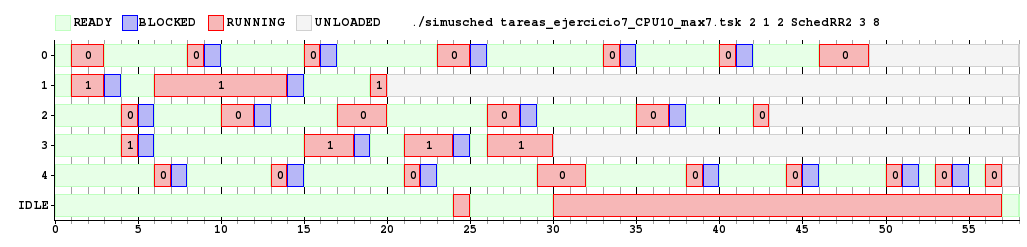
\includegraphics[width=450pt]{./figs/ej8/ej8-c2-q3-8.png}
\end{figure}

\begin{figure}[h]
	\centering                                                       
	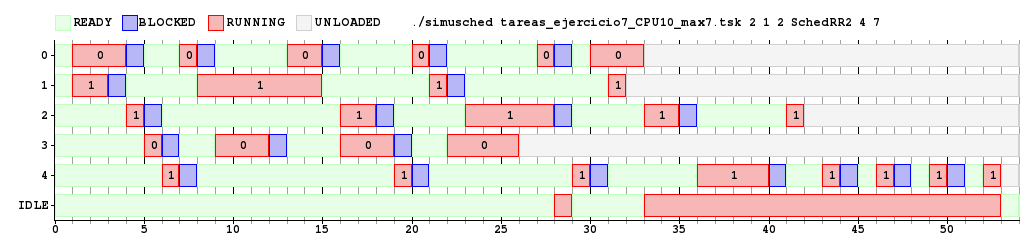
\includegraphics[width=450pt]{./figs/ej8/ej8-c2-q4-7.png}
\end{figure}

\begin{figure}[h]
	\centering                                                       
	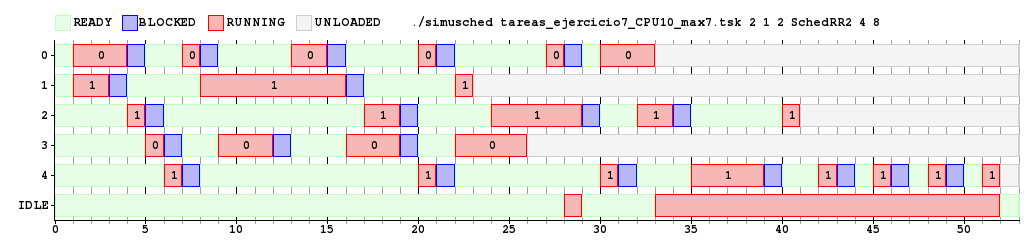
\includegraphics[width=450pt]{./figs/ej8/ej8-c2-q4-8.png}
\end{figure}

\begin{figure}[h]
\centering                                                       
	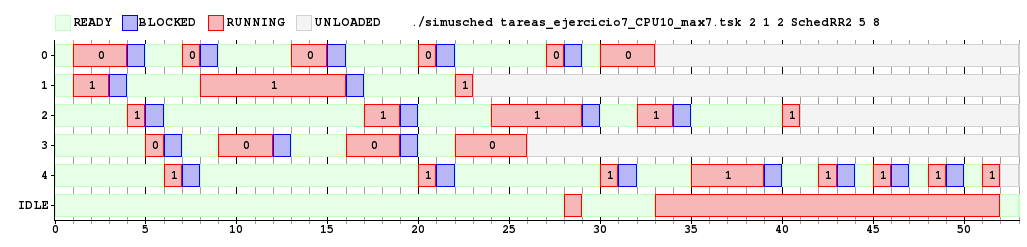
\includegraphics[width=450pt]{./figs/ej8/ej8-c2-q5-8.png}
\end{figure}

\indent De aquí se extrae que, para este lote de tareas, a partir de un quantum igual a cuatro para el core 0, y un quantum igual a 8 para el core 1 se obtiene la misma forma de ejecución si se aumentan los quantums.

\subsubsection{Tres cores}

\indent Análogamente al caso de estudio con 2 cores, se estudiaron casos con los mismos valores de quantum para los tres cores con quantums desde dos hasta diez y se volvió a analizar el turnaround time y el waiting time. A continuación se presentan gráficos para algunos casos:\\ 

\begin{figure}[h]
\centering                                                       
	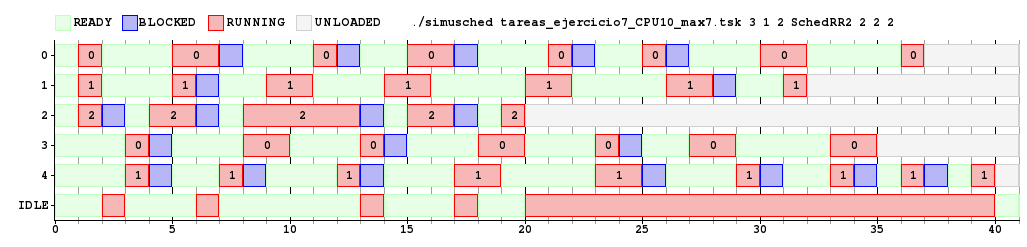
\includegraphics[width=450pt]{./figs/ej8/ej8-c3-q2.png}
\end{figure}

\begin{figure}[h]
\centering                                                       
	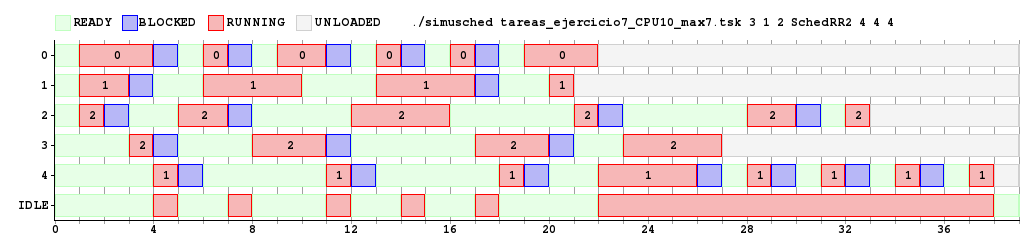
\includegraphics[width=450pt]{./figs/ej8/ej8-c3-q4.png}
\end{figure}

\clearpage

\indent De estos primeros dos gráficos podemos observar como se mejora el tiempo de ejecución para el caso de quantum igual a cuatro con respecto al de quantum igual a 2.\\
\begin{figure}[h]
\centering                                                       
	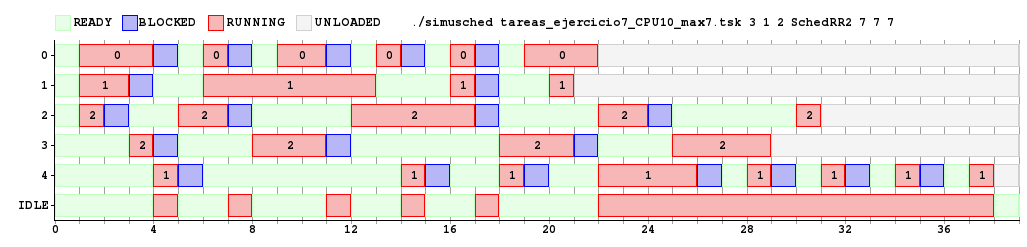
\includegraphics[width=450pt]{./figs/ej8/ej8-c3-q7.png}
\end{figure}

\begin{figure}[h]
\centering                                                       
	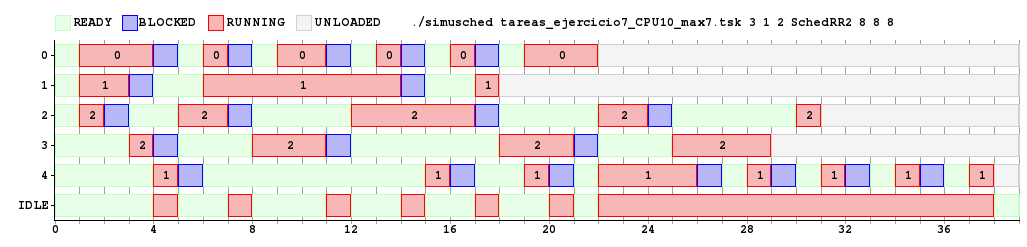
\includegraphics[width=450pt]{./figs/ej8/ej8-c3-q8.png}
\end{figure}

\begin{figure}[h]
\centering                                                       
	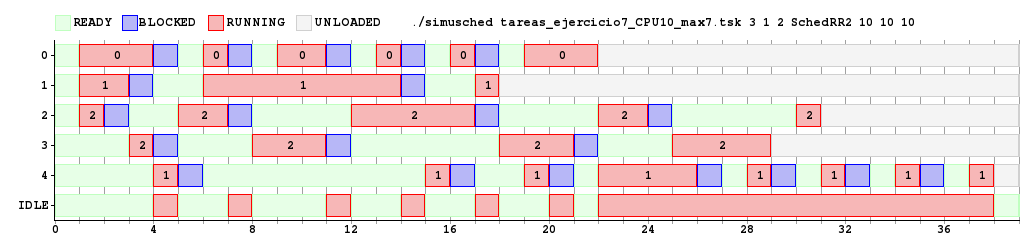
\includegraphics[width=450pt]{./figs/ej8/ej8-c3-q10.png}
\end{figure}

\clearpage

\indent Aquí podemos observar como si bien no se mejora el tiempo total de la ejecución de todas las tareas con respecto al caso con quantum igual a cuatro, si se mejora el de algunas de las tareas que tardan menos en ejecutarse. De la misma manera que en los anteriores casos de estudio, se observa como desde un quantum igual a ocho para los tres cores no varía ni la forma ni el tiempo de ejecución de las tareas.\\

\indent A partir de los casos analizados se generaron gráficos que muestran la variación del turnaround time y del waiting time para las tareas a medida que se aumenta el quantum para los tres cores.\\

\begin{figure}[h]
\centering                                                       
	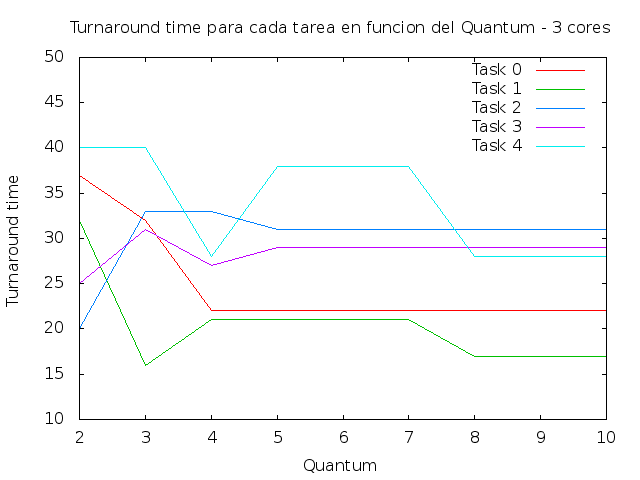
\includegraphics[width=300pt]{./figs/ej8/turnaround3cores.png}
\end{figure}

\begin{figure}[h]
\centering                                                       
	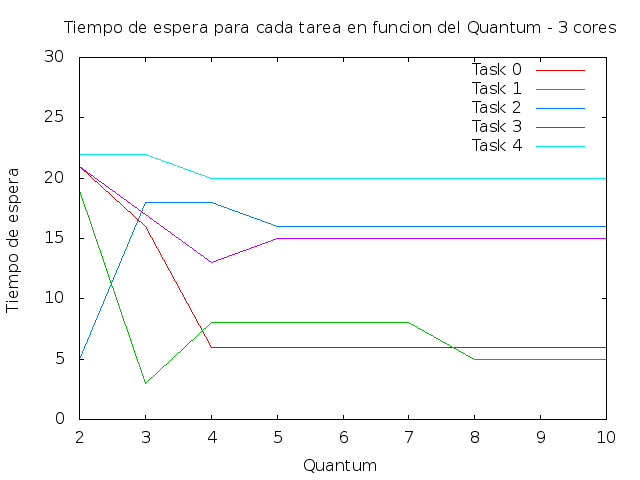
\includegraphics[width=300pt]{./figs/ej8/waitingtime3cores.png}
\end{figure}
\clearpage


\indent De estos gráficos se observa que a pesar de empezar de manera fluctuante, el turnaround time y el waiting time de las tareas se estabiliza a medida que se aumenta el quantum, para algunas antes que para otras.\\


\indent Para el análisis con distintos quantums en cada core, se procedió de la misma manera que cuando estudiamos los casos con dos cores. Los gráficos que se obtuvieron son:\\

\begin{figure}[h]
\centering                                                       
	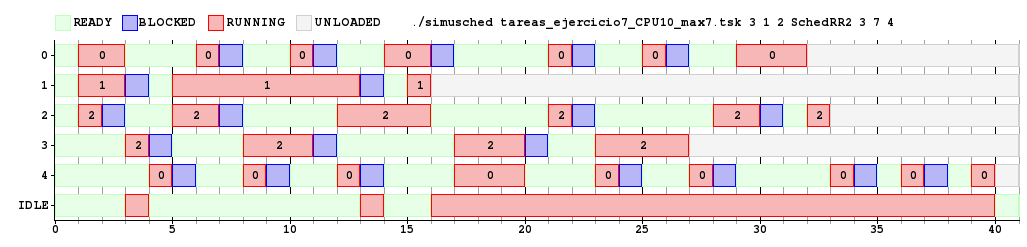
\includegraphics[width=450pt]{./figs/ej8/ej8-c3-q3-7-4.png}
\end{figure}

\begin{figure}[h]
\centering                                                       
	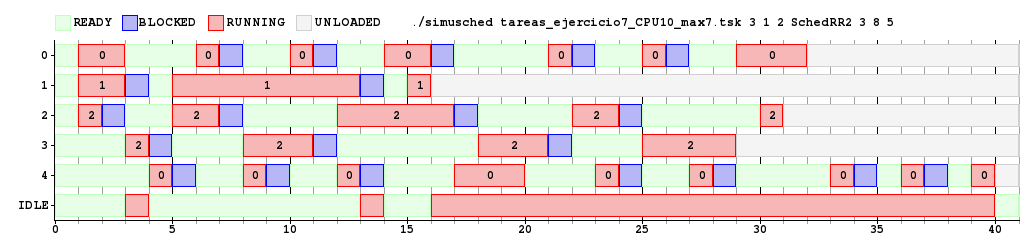
\includegraphics[width=450pt]{./figs/ej8/ej8-c3-q3-8-5.png}
\end{figure}

\begin{figure}[h]
\centering                                                       
	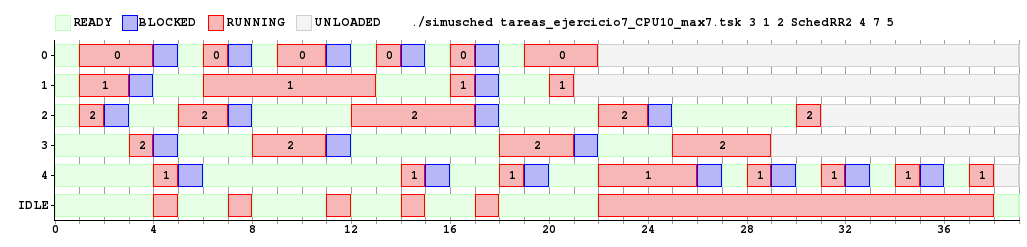
\includegraphics[width=450pt]{./figs/ej8/ej8-c3-q4-7-5.png}
\end{figure}

\begin{figure}[h]
\centering                                                       
	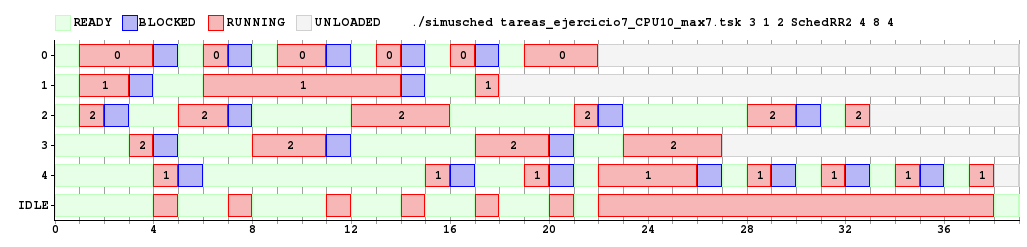
\includegraphics[width=450pt]{./figs/ej8/ej8-c3-q4-8-4.png}
\end{figure}

\begin{figure}[h]
\centering                                                       
	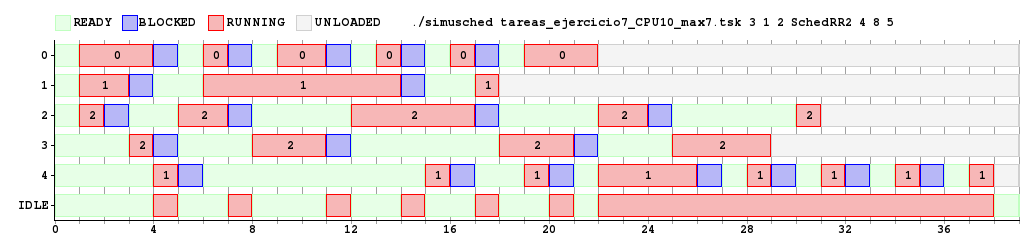
\includegraphics[width=450pt]{./figs/ej8/ej8-c3-q4-8-5.png}
\end{figure}

\clearpage

\indent De estos gráficos podemos observar como la manera en la que actúa cada core parece estabilizarse para cada uno por separado. De esta manera, el caso con quantum igual a cuatro para el core 0, quantum igual a 8 para el core 1 y quantum igual a 5 para el core 2, se nota que el scheduler se comporta de la misma manera que si los tres cores tuvieran quantum igual a ocho, que es el caso desde el cual observamos que se estabilizaba.\\
\indent Es decir que para este lote de tareas, a partir de un quantum igual a 4 para el core 0, un quantum igual a 8 para el core 1 y un quauntum igual a 5 para el core 2 el schedule se comportará de la misma manera.\\

\clearpage

\subsection{Comparación con los criterios del ejercicio 7}

\begin{figure}[h]
	\centering                                                       
	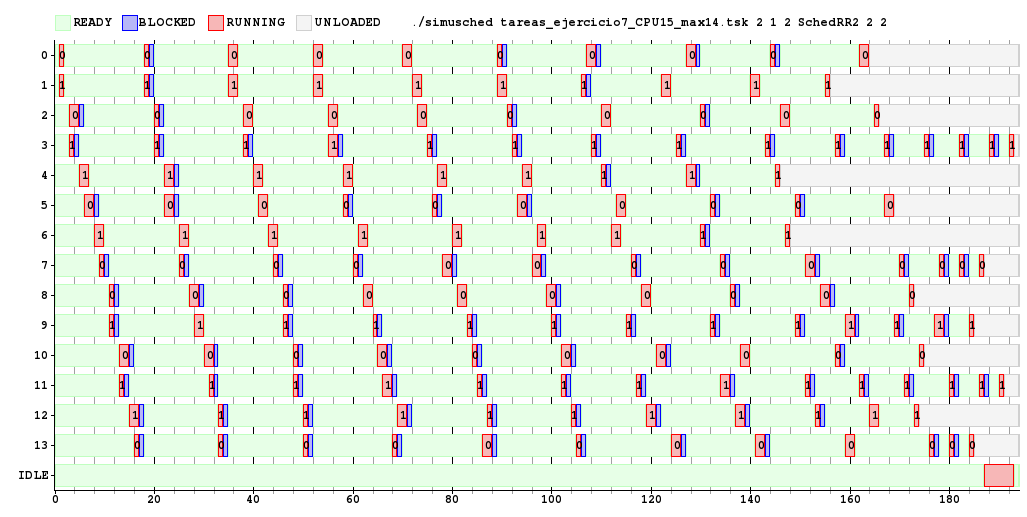
\includegraphics[width=450pt]{./figs/ejercicio8_2cores_quantum2.png}
\end{figure}

Lo que podemos ver al comparar la implementación de \textit{Round Robin 2} a diferencia del ejercicio 7, es que tenemos un algoritmo que no permite la migración de un proceso de un core a otro. Esto trae aparejado tanto ventajas como desventajas. En el primer grupo tenemos la ausencia del costo de migración entre núcleos, porque, lógicamente, dicha penalización no existe. En nuestras pruebas (con los costos de cambio de core y contexto fijados por el enunciado), esta ventaja es evidente cuando el quantum es pequeño, ya que la migración representa un porcentaje más alto de tiempo ``perdido'', en relación a la duración de cada turno para cada tarea. En nuestra experimentación en particular, se puede ver en el ejemplo de 2 cores, que baja el \textit{turnaround time} de aproximadamente 264 ticks a  198.\\
\indent Por otro lado, cuando el quantum no es pequeño, y los procesadores se utilizan de mejor forma, las tareas terminan de ejecutarse antes. Esto hace que la cantidad de veces que se cambia el núcleo de ejecución sean menos, haciendo que si eliminamos ese costo, no estemos mejorando de una manera tan importante el resultado final de la ejecución (es decir, estamos quitando algo que por otras características del experimento, ya no es tan protagonista de las mediciones como antes) como veremos a continuación.

\begin{figure}[h]
	\centering                                                       
	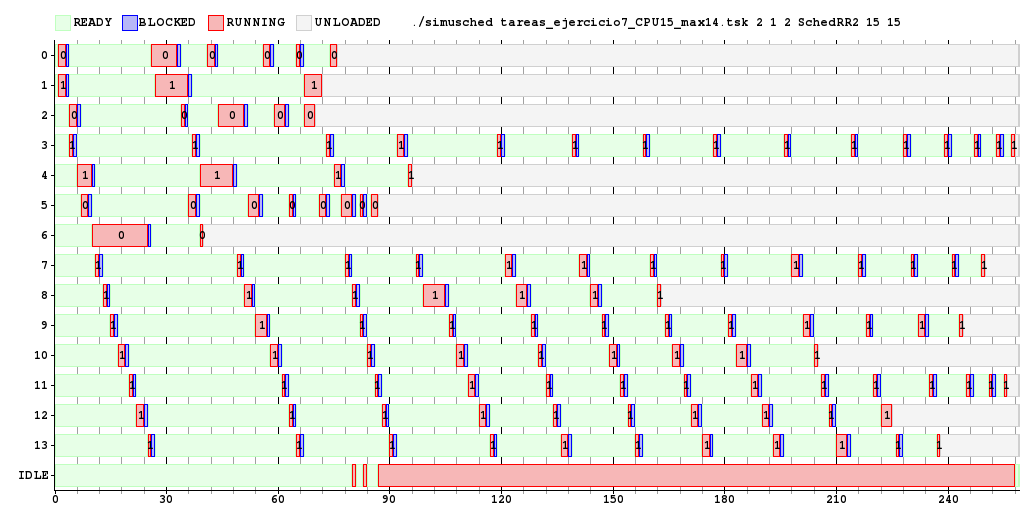
\includegraphics[width=450pt]{./figs/ejercicio8_2cores_quantum15.png}
\end{figure}

\clearpage

Las mejoras dadas por la falta de costo de migración de core no están presentes en el \textit{turnaround time}. No solo eso, sino que por el contrario, el \textit{turnaround time} es peor que en la experimentación con los mismos parámetros, pero con el algoritmo usado en el ejercicio 7.\\
\indent Esto es porque, como dijimos, no se aprovecha la fijación de una tarea con un core. El mayor problema con este enfoque es que uno no sabe de antemano cuanto va a tardar una tarea en terminar, y puede ser que mientras una tarea termina rápido, otra esté en estado \textit{ready}, atada a otro core, esperando su turno, mientras hay otro/s CPU/s en estado idle. Esto hace que el porcentaje de \textit{CPU Utilization} con este escenario disminuya de forma alarmante. Un CPU en estado idle existiendo tareas en estado \textit{ready} es una de las peores cosas que le pueden pasar a un algoritmo de scheduling como los que estamos viendo en este trabajo.

\subsubsection{Conclusiones de este ejercicio}

\indent Como conclusión, es claro que la elección del valor de los quantum para cada core es crucial para el desempeño del scheduler. Para los casos vistos existen valores de quantum a partir de los cuales la manera en la que se comporta el scheduler no cambia. \\
\indent Así, para el caso con un único core alcanza con elegir un quantum igual a 8. Para el caso con dos cores, basta con elegir un quantum igual a cuatro para el core 0, y un quantum igual a ocho para el core 1. Finalmente, para el caso con tres cores, elegir un quantum igual a cuatro para el core 0, un quantum igual a ocho para el core 1 y un quantum igual a 5 para el core 2 es suficiente para obtener los mejores valores de desempeño del scheduler.\\
\indent Nos quisiera mencionar además que la elección del quantum se ve fuertemente influencia por el lote de tareas que se corre. Es decir que no necesariamente estos valores de quantum serán los que mejor se comporten para otros lotes.\\


\newpage

%%%%%%%%%%%%%%%%%%%
%    Ejercicio 9    			   %
%%%%%%%%%%%%%%%%%%%

\section{Ejercicio 9}

Acá va el ejercicio 9
\newpage















%%%%%%%%%%%%%%%%%%%%%%%%%%%%%%%%%%%%%%%%
%        Esto es de mi template        %
%    Dejar para futuras referencias    %
%%%%%%%%%%%%%%%%%%%%%%%%%%%%%%%%%%%%%%%%

% \section{Sección, título grande}
% \\
% \textcolor{white}{Sarasa engañadora de formato, jua jua}\\
% Esto es texto. Con doble barra invertida es el enter.
% \\
% \\
% \textit{De acá en adelante, todo lo que se explica como "para hacer x se usa y", implica que antes de y va una barra invertida}
% \\
% \\
% Con \textbf{textbf\{\}} se escribe en negrita.
% \\
% \\
% \section{Bullet \& Numbering}
% Para hacer items se usa \textbf{begin\{itemize\}} y \textbf{end\{itemize\}}, por ejemplo:
% \begin{itemize}
% 	\item Esto es un ítem.
% 	\item Esto es otro.
% \end{itemize}
% Con \textbf{item} se hace cada uno de los ítems. Si cambiás \textbf{itemize} por \textbf{enumerate} te lo hace enumerado. Por ejemplo:
% \begin{enumerate}
% 	\item Acá está el primero.
% 	\item Acá el segundo.
% \end{enumerate}
% \\
% Y así.
% \\
% \\
% \section{Tablas}
% También tenemos las tablas, que son un poco más rebuscadas. Se usa \textbf{begin\{tabular\}\{cols\}} y en cols ponemos c si queremos una columna centrada, l y r
% para otro tipo de justificación. Si las c las separás con espacios, se hacen columnas sin división. Si ponés un pipe es con una línea divisoria, dos pipes con
% dos líneas, y así. Se termina con \textbf{end\{tabular\}}. Para separar entre elementos de fila/columna se usa un ampersand (\&, y es necesario para separar
% elementos entre filas y columnas, no solo entre filas) y para cambiar de fila \textbf{SIN} linea divisoria, un \textbf{newline} ya que el doble barra invertida
% te hace un enter dentro de la celda. Con línea divisoria es reemplazando \textbf{newline} por \textbf{hline}.
% \\
% \\
% Más datos en el principio de este tex. Un ejemplo:
% \\
% \\
% \begin{tabular}{| c| c|}\hline
%     Celda 1 & Celda 2 &\hline
%     Celda 3 & Celda 4 &\hline
% \end{tabular}
% \\
% \\
% \section{Verbatim}
% \begin{verbatim}
% Esto es verbatim. Es un entorno que no le da ni 5 de pelota al formato de latex.
% Por eso mismo hay que tener cuidado con no irse de la hoja o similar.
% Sirve por ejemplo, para pseudocódigo:
% 
% if (se cumple sarasa){
%     ejecuto cosito1;
%     ejecuto cosito2:
% }else{
%     ejecuto cosito3:
% }
% \end{verbatim}

\end{document}
